\documentclass[10pt]{article}
\usepackage[a4paper,margin=24mm]{geometry}
\usepackage{amsmath,amssymb,amsthm,booktabs,graphicx,array,longtable}
\usepackage[T1]{fontenc}
\usepackage{lmodern,microtype,xcolor}
\usepackage[colorlinks=true,linkcolor=blue!45!black,citecolor=blue!45!black,urlcolor=blue!45!black]{hyperref}
\usepackage{xurl}
\setlength{\emergencystretch}{2em}
\usepackage{natbib}
\setlength{\parskip}{3pt}
\setlength{\parindent}{0pt}
\newcommand{\R}{\mathbb{R}}
\newcommand{\E}{\mathbb{E}}
\newcommand{\Cov}{\operatorname{Cov}}
\newcommand{\norm}[1]{\left\lVert#1\right\rVert}
\newcommand{\src}[2]{\href{../../../#1}{#2}}
\newtheorem{proposition}{Proposition}
\title{What Does Temporal Gradient-Subspace Filtering Select?\\[5pt]\large Conditional protection, sampler effects, and a local observer-history pathway}
\author{Internal working draft prepared for the project owner\\\small Analysis and manuscript assembly: Codex}
\date{10 September 2026}
\begin{document}
\maketitle
\begin{abstract}
Restricting learning to a subspace of past gradient variation can preserve useful behavior, but variation is not a label for usefulness. We characterize a temporal gradient-covariance filter through three connected studies. In a three-seed MNIST experiment, stable filtering preserves common-digit accuracy under diffuse label corruption: 62.01\% versus 33.97\% for raw AdamW. This benefit coexists with zero recognition of a newly introduced rare correct class and a largely learned misleading patch cue, despite partial cue protection. A separate three-seed intervention rearranges the same indexed example occurrences and assigned labels within fixed blocks. Grouping strengthens noisy common-accuracy preservation in every seed without restoring rare recognition. Holding model parameters, Adam state and action input fixed then identifies a local observer-history pathway. Grouping improves relative rare loss in all three reused Clean parents, but only one of three Diffuse parents; increased access to the rare probe direction is insufficient for improved delivered alignment. Complementary five-seed modular-addition branches support useful directional restriction against a specified raw-direction policy, with legacy/stable and elapsed-time qualifications. A selective-continuation construction explains why directional restriction can outperform global stopping under favorable assumptions. The empirical contribution is a conditional learning tradeoff and a controlled local pathway, not a new covariance identity, a universal optimizer advantage or a demonstrated alignment intervention.
\end{abstract}

\section{Introduction}
Training interventions intended to resist undesirable learning must preserve useful prior knowledge without preventing legitimate adaptation. This is a safety-relevant problem: competent behavior can generalize toward unintended goals, rather than merely fail through incapacity \citep{shah2022goals}. Our classifiers are not agents and do not test goal misgeneralization. We study a narrower prerequisite: whether update restriction preserves useful predictions while limiting unwanted associations, and when the same restriction blocks rare correct learning or admits a coherent misleading feature.

Random-label fitting motivates this question \citep{zhang2017rethinking}, as do limitations of tightly restricted two-sided uniform-convergence bounds in specific constructions \citep{nagarajan2021uniform}. Neither says useful theory is impossible: surrogate-based analyses give guarantees in related settings \citep{negrea2020defense}. We seek conditional, testable relationships between learning dynamics and behavior, consistent with the constructive program of \citet{simon2026theory}; changing an optimizer is not itself an explanation of ordinary SGD. Coherent Gradients and subspace methods already supply direct precedents. Our question is what one temporal observer permits, how presentation changes that behavior, and which local response can be attributed to its history.

The answer has a positive and a limiting part. Filtering can preserve common recognition against diffuse corruption, and a separate rule-learning intervention can improve generalization despite a raw alternative fitting the training set perfectly. These are useful changes in learning. They do not amount to semantic selection: the MNIST policy restricts new rare recognition and still learns a strong wrong cue. Moreover, the sampler changes the tradeoff even when total indexed exposure is conserved. A local experiment then shows that greater access to a helpful probe direction does not determine useful delivery of the current mixture.

Table~\ref{tab:headline} gives the three primary findings and their paired limits. We separate the temporal statistic, delivered gradient and actual Adam displacement. Appendix~\ref{app:ledger} retains complementary and contradictory studies; Appendix~\ref{app:ordinary-augmentation} adds completed ordinary-augmentation comparisons. Native policies keep learning, including strong rank-200 noisy-label gains, but augmented raw AdamW remains substantially better in both tested configurations. No experiment was rerun for this source-linked working synthesis; it is neither a submission nor an established-priority claim.

\begin{table}[t]
\centering\small
\begin{tabular}{>{\raggedright\arraybackslash}p{.24\linewidth}>{\raggedright\arraybackslash}p{.32\linewidth}>{\raggedright\arraybackslash}p{.35\linewidth}}
\toprule
Study and replication & Positive observation & Boundary beside the observation\\\midrule
Selectivity, 3 paired seeds & Diffuse common accuracy: 62.01\% native vs.\ 33.97\% raw & Rare accuracy: 0\% vs.\ 51.73\%; both lose common accuracy from warmup\\
Shared cue, same 3 seeds & Cue-interaction reduction: 3.358 points, favorable in every seed & Native patch excess remains 94.825 points; misleading association is learned\\
Batching, 3 fresh paired seeds & Grouped native noisy common accuracy: 56.64\% vs.\ 47.92\% interleaved & Native rare accuracy remains 0\% in every noisy branch\\
Observer histories, 3 reused parents & Clean rare loss contrast: $+0.003092\pm0.000894$ nats/example & Diffuse: $-0.000616\pm0.000711$; local, outcome-informed study\\
Grokking branch, 5 parents & Raw minus projected final CE: $+3.8245\pm0.6632$ & Inherited legacy state; same functional norm rule, not identical scale histories\\\bottomrule
\end{tabular}
\caption{Headline evidence, with limits that change its interpretation. Native here means the stable rank-32 policy; the grokking branch uses a different legacy rank-200 observer. Errors are sample SE across the stated paired seeds or reused parents, not confidence intervals. CE is cross-entropy; positive observer utility means loss reduction. Studies are not pooled replicates. Direct sources are mapped in Appendix~\ref{app:sources}.}
\label{tab:headline}
\end{table}

\section{The constructive case and the actual operator}
\subsection{Selective continuation can exceed global stopping}
Consider fixed-design linear regression with training loss $L_{\mathrm{tr}}(\theta)=\frac{\lambda}{2}\norm{\theta-w}^2$, where $w=\theta^*+\zeta$ is a noisy training optimum. Clean risk is $R(\theta)=\frac{\lambda}{2}\norm{\theta-\theta^*}^2$. Suppose $\theta^*\perp\zeta$, with $A=\norm{\theta^*}^2>0$ and $B=\norm{\zeta}^2>0$. Starting at zero, ordinary gradient descent with an isotropic Hessian follows a scalar multiple of $w$. Even allowing every real scalar endpoint gives
\begin{align}
R(\alpha w)&=\frac{\lambda}{2}\left[A(1-\alpha)^2+B\alpha^2\right],\\
\min_{\alpha\in\R}R(\alpha w)&=\frac{\lambda}{2}\frac{AB}{A+B}>0.
\end{align}
An orthogonal projector $\Pi$ that retains $\theta^*$ and removes $\zeta$ instead permits continuing useful learning:
\begin{equation}
\theta_{t+1}=\theta_t-\eta\Pi\nabla L_{\mathrm{tr}}(\theta_t),\qquad
R(\theta_t)=\frac{\lambda A}{2}(1-\eta\lambda)^{2t}\longrightarrow0
\end{equation}
for $0<\eta\lambda<1$. This follows directly by induction on the retained component. The construction gives a strict advantage over global scalar stopping or shrinkage under its assumptions. It does not show that a temporal observer discovers the helpful projector, or beat a comparator already supplied with that projector. This standard conditional argument is a steelman for the experiment, not a claimed new theorem. The existing derivation also treats imperfect directions and explains why isotropic full-batch covariance need not discover the useful space.

\subsection{Centering, finite memory and self-inclusion}
Let $g_t\in\R^P$ be a flattened batch-mean parameter gradient. The intended observer updates its mean before computing an innovation:
\begin{equation}
\mu_t=\beta\mu_{t-1}+(1-\beta)g_t,\quad
z_t=g_t-\mu_t,\quad
C_t\simeq\beta C_{t-1}+(1-\beta)z_tz_t^\top.
\label{eq:observer}
\end{equation}
The approximation matters. The implementation stores a $P\times k$ factor and smaller state; repeated truncation, finite precision and special initialization prevent interpreting it as an exact full-history covariance. The mean is seeded by the first gradient. The first nonzero innovation initializes its singular scale to $\norm{z}$ without the later $(1-\beta)$ weighting. Current gradients are observed before the action, so the observer is causal but includes the current input rather than depending exclusively on the strict past.

Centering is also different from agreement. If $g_i=s+\epsilon_i$ at fixed parameters with zero-mean $\epsilon_i$, then $\Cov(g_i)=\Cov(\epsilon_i)$, whereas $\E[g_ig_i^\top]=ss^\top+\Cov(\epsilon_i)$. A perfectly shared component can be absent from centered covariance; finite initialization transients can still reveal it. Across training time, the gradients additionally change with the model. Neither a covariance direction nor its variance is intrinsically a semantic feature.

\subsection{A supplied gradient is not the resulting parameter step}
The native hard action is $h=VV^\top g$, with an identity fallback before a basis exists. Orthonormal $V$ makes this projection. A legacy nonorthogonal basis, written $V=Q\Sigma W^\top$, instead gives $h=Q\Sigma^2Q^\top g$: its span and its within-span gains are distinct. The stable MNIST policy uses numerical repair; the legacy grokking evidence must not be described as the same ideal projector.

Both feed ambient-coordinate AdamW. Writing $v_t$ for its coordinatewise second moment, the actual displacement is
\begin{align}
m_t&=\beta_1m_{t-1}+(1-\beta_1)h_t,\qquad
v_t=\beta_2v_{t-1}+(1-\beta_2)h_t^{\odot2},\\
\Delta\theta_t&=-\eta\frac{\widehat m_t}{\sqrt{\widehat v_t}+\epsilon}-\eta\lambda_{\rm wd}\theta_{t-1}.
\end{align}
Coordinatewise division, inherited moments and weight decay need not preserve the delivered subspace. Supplying an explicit zero gradient still advances moments and applies decay; it is not a skipped update. Likewise, matching $\norm{h_t}$ need not match the norm or direction of $\Delta\theta_t$. Our controls and interpretations preserve these distinctions.

\section{Useful protection with rare-learning and cue costs}
\label{sec:select}
The first primary study uses three paired seeds and 36 continuations of a 784--64--10 ReLU MLP. A clean 100-step AdamW warmup learns nine MNIST digits but excludes digit 8. Later training includes 50 correct digit-8 images among 5,000 images. Every continuation restores the same warmup model, Adam, observer and random state within seed and runs to absolute step 2,000. The held-out set is disjoint from training and comes from the official training files; the official test split is unused. Appendix~\ref{app:methods} gives the exact recipe.

We compare raw AdamW, stable global rank-32 filtering, and an own-state norm rule along raw direction. Four conditions distinguish clean data, diffuse majority-label corruption, a shared misleading patch and its matched sham. Rare labels remain correct and rare training images remain unpatched. Under Diffuse, each majority example is selected with probability 0.9 for uniform replacement among nine non-8 labels, including the original label: the expected changed-label fraction is 0.8, not 0.9.

The useful result is substantial common-digit accuracy preservation: 62.01\% native versus 33.97\% raw, with paired gains of 28.18, 23.38 and 32.56 percentage points. Wrong-target training accuracy is 6.22\% versus 32.48\%. These outcomes jointly show retained useful classification with reduced corrupted-target fitting. They are not simply a high covariance reconstruction score.

The change from warmup qualifies the mechanism. Common warmup accuracy is 87.76\%, so both policies deteriorate; native loses less. Common CE is 1.8750 versus 1.8741, nearly unchanged in mean with mixed paired signs, and balanced CE is worse for native. Better accuracy is not uniformly better probability prediction. Rare recognition is also substantially restricted: Clean native accuracy is 4.93\% versus 52.00\% raw; Diffuse is 0\% versus 51.73\%. Yet native rare CE improves from warmup in every cell and seed. Zero argmax accuracy is therefore not zero learning or a frozen model.

\begin{figure}[t]
\centering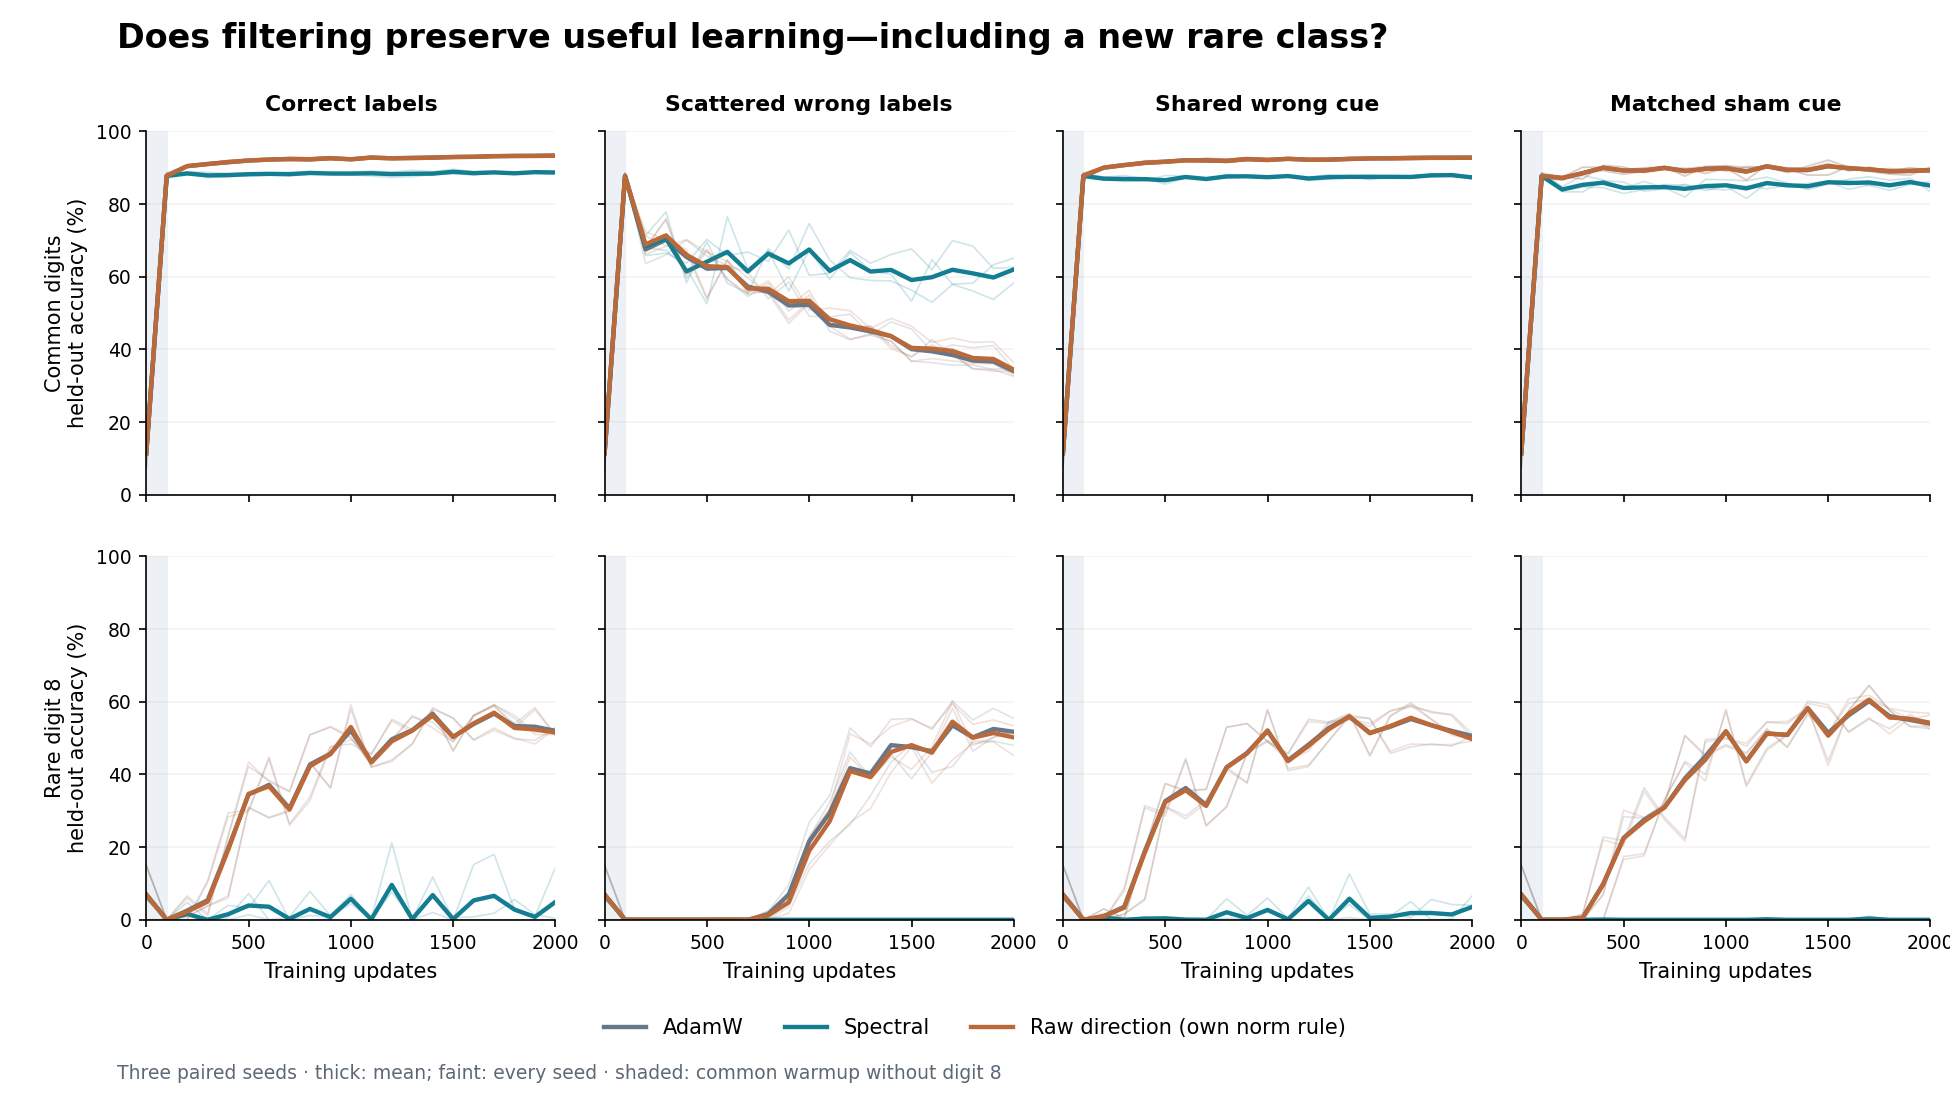
\includegraphics[width=\linewidth]{../../2026-09-09-spectral-selectivity-boundary/results/learning.png}
\caption{Preservation and acquisition differ. Existing all-seed curves from the selectivity study show common and rare accuracy under its four conditions. Native noisy common accuracy declines less than raw, while rare recognition is strongly restricted. The rare class was excluded from warmup; frequency, novelty and digit identity are entangled.}
\label{fig:learning}
\end{figure}

The shared-cue condition assigns target 0 to 500 true-nonzero majority images and adds a white upper-left $3\times3$ patch. The sham preserves assigned labels and total/per-digit patch counts but reallocates patches approximately independently of poison status within true digit. On 4,000 matched held-out nonzero common images, define $E$ as patched minus unpatched target-0 prediction rate. The registered interaction is
\begin{equation}
D_{\rm cue}=[E_{\mathrm{native,Shared}}-E_{\mathrm{native,Sham}}]
-[E_{\mathrm{raw,Shared}}-E_{\mathrm{raw,Sham}}].
\end{equation}
Native reduces it by $3.358\pm0.893$ points, favorable in all three seeds. Shared patched common CE is also much lower: 2.9232 versus 11.3060. Nevertheless, native Shared patch excess remains 94.825 points, and wrong-target fitting is 96.87\%. This is partial protection against confident cue errors alongside a readily learned misleading association, not absence of protection or rejection of the cue.

The own-norm raw policy largely resembles raw AdamW. Its specified scalar rule does not reproduce this tradeoff, although it does not match realized scales or Adam displacements between trajectories. Sparse diagnostics further weaken a permanent-exclusion account: late Clean/Shared rare mean-action energy retention reaches 98.05--99.12\% despite poor rare recognition. These probes do not identify which intervening updates cause the endpoint cost. The observed boundary is behavioral; it is not an inference that every helpful rare direction was discarded.

A subsequent three-seed augmentation study (Appendix~\ref{app:augmentation}) adds a learning boundary: random masking improves raw rare learning but worsens native rare CE, while targeted cue erasure changes cue contrasts with competence costs. Native nevertheless retains relative patched-image protection. Lower cue frequency does not make a surviving cue unreliable.

\section{The same exposure produces a different tradeoff}
\label{sec:batch}
The second study uses three fresh paired seeds, the same architecture and optimizer recipe, and 36 continuations crossing Clean/Diffuse, two schedules and three policies. Each 50-update block contains exactly the same 3,200 indexed image occurrences, including repetitions and assigned labels, under both schedules. Interleaved distributes rare occurrences nearly evenly; Grouped packs them into fewer batches. Neither schedule is the older iid schedule. There is no added rare weight or oversampling.

At fixed parameters, let $D$ contain indexed per-example gradients and $w_t$ their batch weights. Then
\begin{equation}
g_t=Dw_t,\qquad \Cov(g_t)=D\Cov(w_t)D^\top.
\end{equation}
Equal mean exposure does not determine covariance. For two deterministic groups,
\begin{equation}
g_t=\mu_c+q_t(\mu_r-\mu_c),\qquad
\Cov(g_t)=\operatorname{Var}(q_t)(\mu_r-\mu_c)(\mu_r-\mu_c)^\top.
\end{equation}
The salient direction is a group contrast, not automatically the rare mean or its useful component. These standard identities motivate changing presentation. They do not describe exactly the centered, rank-truncated moving observer, and they do not remove ordinary Adam batching effects.

Grouping increases native Diffuse common accuracy from 47.92\% to 56.64\%, with paired gains 9.20, 10.07 and 6.91 points. The native-minus-raw schedule interaction is $8.34\pm1.08$ points and favorable in every seed. Wrong-target fit falls from 7.93\% to 6.40\%; balanced accuracy and CE improve in all three seeds. Common CE is mixed across seeds and remains worse than raw in mean. This is an additional useful preservation effect from rearranging identical exposure.

\begin{figure}[t]
\centering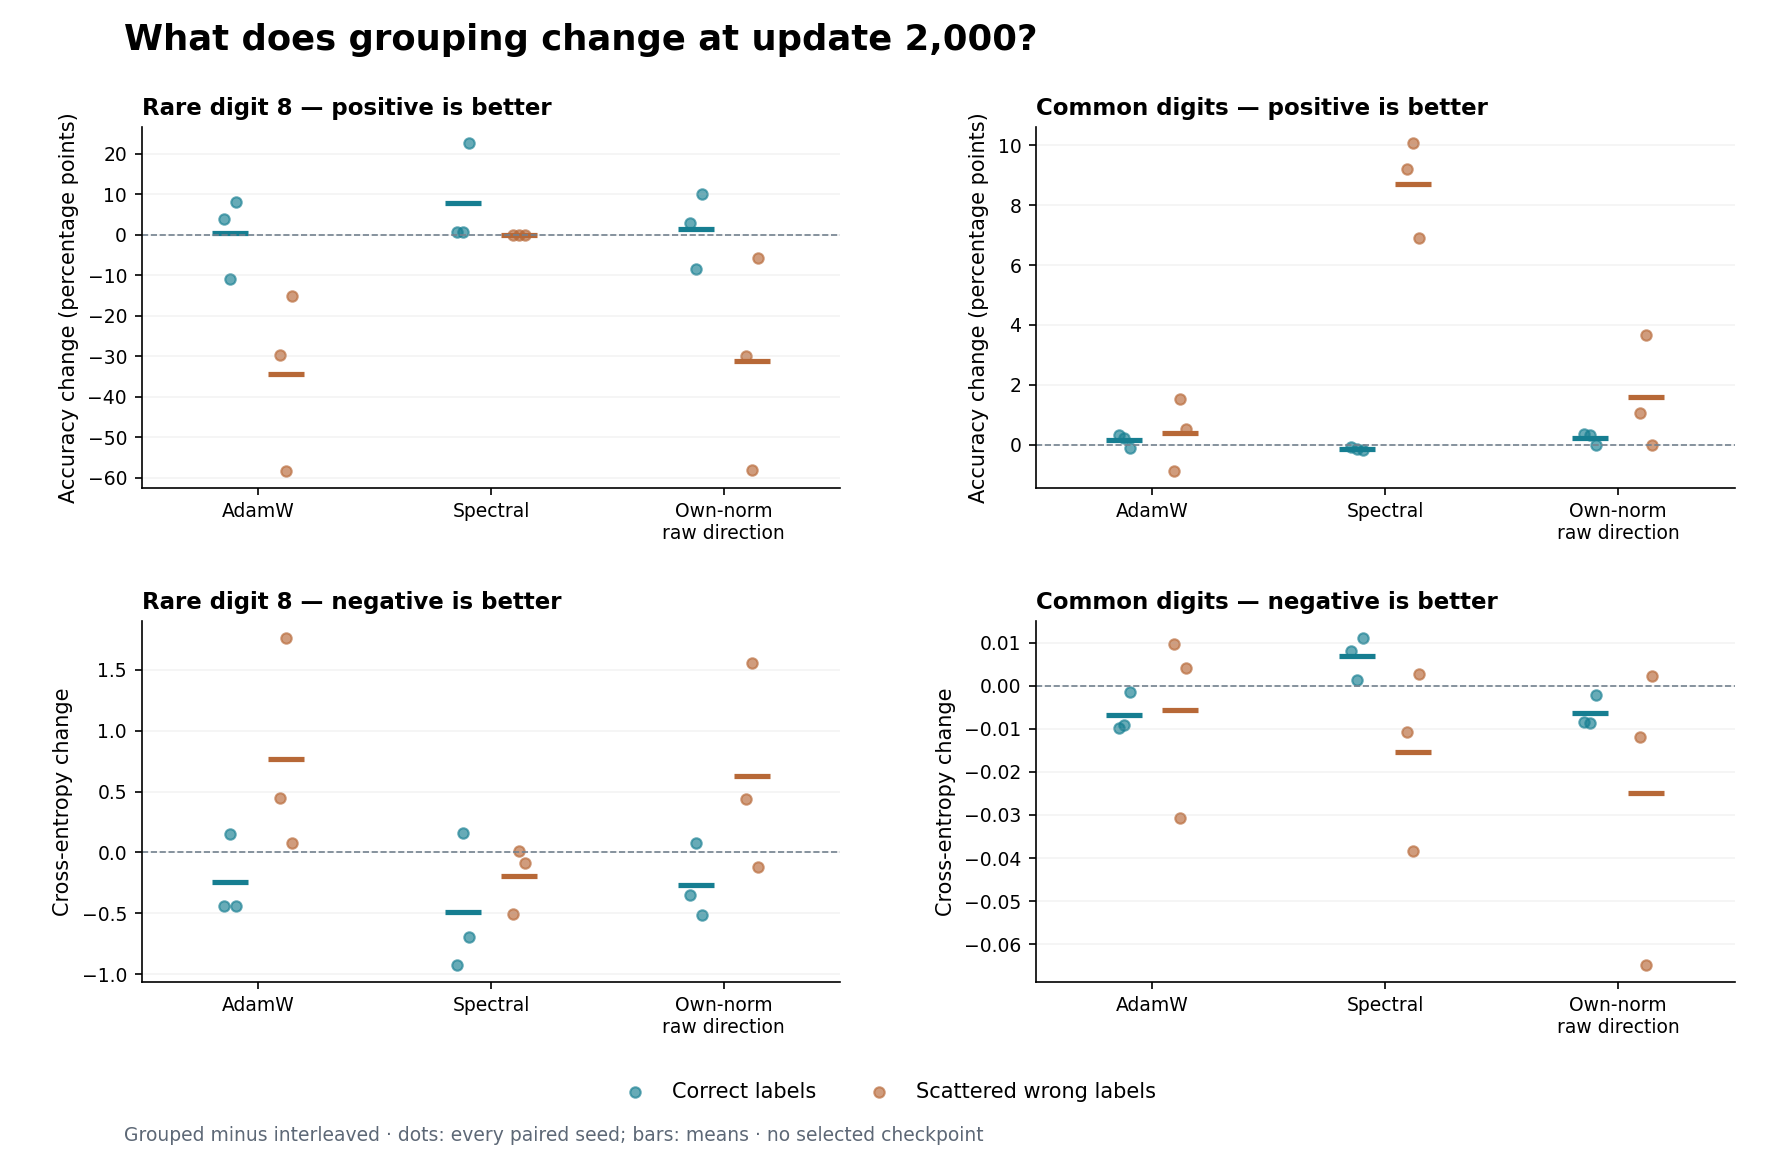
\includegraphics[width=\linewidth]{../../2026-09-10-spectral-batch-composition/results/schedule-effects.png}
\caption{All paired schedule effects from the equal-exposure study. Grouping improves native noisy common accuracy in every seed. Noisy native rare accuracy remains zero. Clean rare gains are uneven and incur common-class costs; favorable difference-in-differences must be interpreted with absolute outcomes.}
\label{fig:batch}
\end{figure}

Rare Diffuse accuracy remains zero in every native branch. The favorable 34.4-point rare-accuracy interaction comes entirely from raw deteriorating from 51.80\% to 17.40\%, not a native rescue. Under Clean, native rare accuracy rises from 2.27\% to 10.27\%, but paired gains are 0.8, 0.6 and 22.6 points; the mean is dominated by one seed. Common accuracy falls and common CE rises in every Clean native comparison. Both raw policies remain better on every Clean rare/common primary.

All 18 registered Grouped high-count events improve the rare training-probe CE after their actual Adam steps. All nine Diffuse high-count events worsen common-probe CE even though grouping improves the common endpoint. Late rare mean-action retention is 96.29--99.18\% despite zero final rare recognition. Helpful individual bursts and poor accumulated recognition can coexist. Sparse event measurements do not determine inter-burst forgetting or endpoint mediation. The established effect is a sampler--policy interaction; the next experiment isolates one local observer-history pathway.

\section{Access, delivery and actual motion}
\label{sec:observer}
The third study reuses the three step-100 parents of Section~\ref{sec:batch} after its outcomes were known. For each Clean/Diffuse cell, two observer copies receive the first 50 grouped/interleaved batch gradients at the same frozen model. No model or Adam update occurs during those histories. The paired block means agree within a predeclared FP32 tolerance; both arms then receive exactly the same float32 input $g^*$, constructed symmetrically from their FP64 means.

Each observer sees $g^*$ once before delivery. Observer time is thus 151 while Adam remains at 100. Native Grouped, native Interleaved, raw $g^*$ and explicit zero each take one step from fresh copies of that model/Adam state. Shared zero steps across label cells give 21 physical steps and 24 logical action/cell entries. This is an artificial local intervention using a smoothed block input, not ordinary next-minibatch continuation or fresh replication of the long-run result.

For a fixed true-label training-probe gradient $q$, these quantities answer different questions:
\begin{align}
\text{access: }&\quad \norm{\Pi q}^2/\norm{q}^2,
&\text{input: }&\quad B_q=q^\top g^*,\\
\text{delivery: }&\quad F_{q,s}=q^\top h_s,
&\text{Adam utility: }&\quad J_{q,s}=-q^\top\Delta\theta_s,\\
\text{held-out utility: }&\quad U_s=L_{\rm hold}(\theta)-L_{\rm hold}(\theta+\Delta\theta_s).
\end{align}
Access concerns a possible direction; delivery depends on its cross term with the actual input. Even for an ideal orthogonal projector, $q^\top\Pi g=(\Pi q)^\top g$ is not determined by $\norm{\Pi q}$. We measure the actual stored native action rather than substitute an ideal projector. The probe contains 32 rare or 54 common training examples, whereas $U$ is held-out CE. Their agreement is not a Taylor decomposition of the same population loss.

Grouped-minus-Interleaved rare held-out utility in Clean is +0.001414, +0.004464 and +0.003399 nats/example. Grouped absolute utilities are $-0.012301$, +0.007962 and +0.025786: two greater improvements and one reduction in damage. In Diffuse the relative contrast is +0.000752, $-0.000962$ and $-0.001638$, despite positive Grouped absolute rare utility in every parent. Rare-probe access rises from 84.5--91.4\% to 98.3--99.1\% in Clean and from 26.3--34.8\% to 97.2--98.6\% in Diffuse. Increased access alone therefore does not order useful noisy delivery.

\begin{figure}[t]
\centering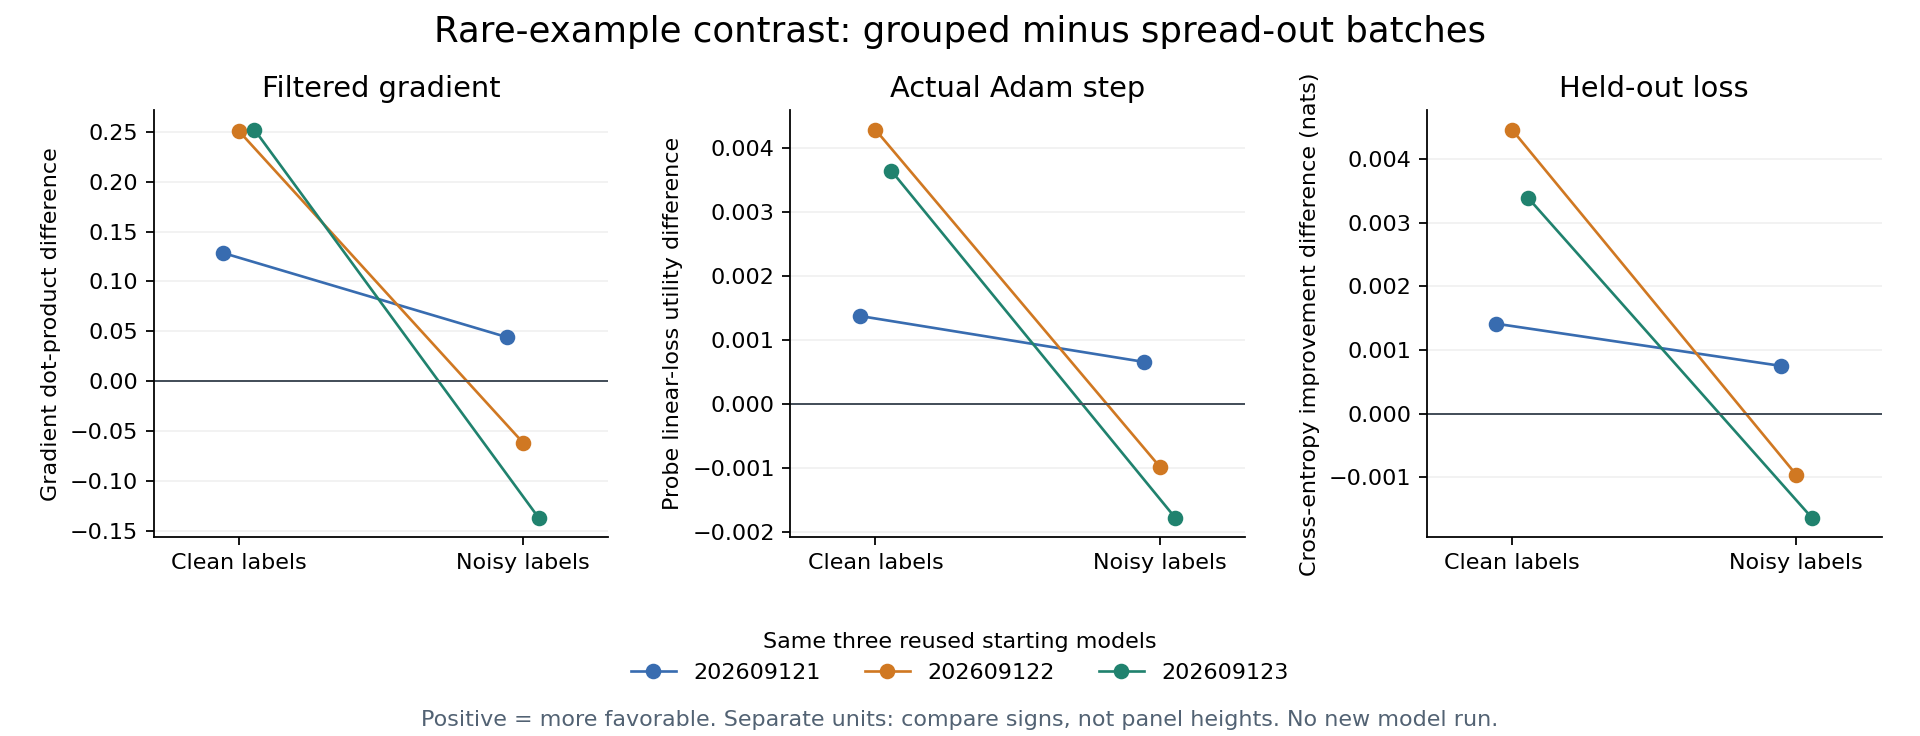
\includegraphics[width=\linewidth]{../../2026-09-10-spectral-observer-signal/results/rare-signal-chain.png}
\caption{The rare grouping contrast across delivery, actual Adam movement and held-out loss, using saved vectors and previously checked outcomes. All six signs agree, with different units at different stages. In two Diffuse parents the adverse relative ordering is already present at delivery. These are three reused parents, not six independent replications; the later vector accounting has internal numerical checks, not a new independent scientific audit.}
\label{fig:chain}
\end{figure}

A subsequent saved-vector calculation supplies the missing cross terms without rerunning a model. Rare $B_q$ is positive in all six cells. Its mean rises from 2.2989 Clean to 4.8866 Diffuse, while cosine falls from 0.4210 to 0.1698; increased absolute dot product is not improved orientation. Grouped-minus-Interleaved delivered alignment is $+0.128563,+0.250851,+0.252053$ in Clean and $+0.044021,-0.061640,-0.136978$ in Diffuse. These signs match the corresponding actual Adam and held-out contrasts. The two adverse noisy relative orderings therefore occur before Adam, not first in its coordinate transformation. All native rare delivered dots remain positive: the adverse relative effect is not absolute negative alignment.

This statement is specific to the rare grouping contrast. Grouped-minus-raw comparisons do reverse order through Adam. Diffuse common delivered dots are negative while actual common Adam and held-out utilities remain positive. Explicit-zero Adam improves common loss and worsens rare loss in every parent; all nonzero actions beat zero on rare utility. Raw improves common held-out CE more than either native history in every cell. Actual native adaptive displacement has 84.84--95.39\% of squared norm outside the observer span. These controls show why delivered projection is not confinement of actual motion or a decomposition of momentum's causal contribution. Rare accuracy remains zero throughout this one-step study, and nonzero Diffuse actions improve wrong-target fitting loss. The local pathway is real but does not establish long-run corruption suppression or explain the step-2,000 ranking.

\section{Complementary evidence and nearest-method scope}
\label{sec:complement}
\subsection{Grokking supports a conditional directional effect}
Five fresh paired modular-addition seeds reach sustained 90\% held-out accuracy at mean steps 2,810 under legacy filtering versus 4,040 with AdamW. The stable implementation reaches 3,980, with substantial variation; its earlier first-crossing mean of 3,460 is not a reliable sustained gain. Both filters take more measured training time than AdamW in every pair. All final accuracies reach 100\%. The constructive learning effect is task- and implementation-specific, not a speed record or a higher final accuracy ceiling.

Branches from complete legacy step-1,500 states separate native $VV^\top g$, orthogonal $\Pi g$ and norm-restored $c\Pi g$, where $c=\norm{VV^\top g}/\norm{\Pi g}$. Plain projection loses to native at both fixed endpoints. Norm restoration improves all final CE, margin and selected representation-readability primaries against native; earlier behavioral signs are mixed. A further raw-direction arm supplies $a g/\norm{g}$ with $a=\norm{VV^\top g}$ recomputed on its own trajectory. At step 2,500 it loses to norm-restored projection on every primary in every seed, despite 100\% training accuracy and only 0.22--2.13\% held-out accuracy. This supports useful directional restriction against that specified functional norm rule, not every scalar controller or the necessity of an adaptively learned span.

At a common nondegenerate state, let $\rho=\norm{\Pi g}/\norm{g}>0$. Norm-restored projection removes the off-span incoming-gradient component and increases retained drive by $1/\rho$ relative to an equal-total-norm raw action. This identity concerns delivered gradients, not actual Adam displacement. A separate one-step functional comparison finds that suppression locally helps held-out CE while hurting training, and amplification partly reverses that benefit. Signed within-sum utility, rather than increased useful sum-consistent motion, carries the local gain. This does not identify a rule circuit, memorization or mediation of the later trajectory. Representation $R^2$ measures linear readability, not an identified mechanism.

\subsection{Competitive scalar controls and prior ideas constrain the claim}
Separate SGDm studies preserve important counterevidence. A scalar temporal-response family is favorable on seven of eight registered mean selector effects in one reused MNIST panel. Gain normalization substantially improves the spectral comparator in a subsequent study, but six of eight joint-selected means still favor scalar, including every fixed-target comparison. Unequal dose, adaptive panel reuse and unequal selection opportunities prevent equivalence claims. They nevertheless rule out presenting projection as generally necessary for the observed protection. Mean-preserving variants can restore useful adaptation while also restoring corrupted-realization fitting, and filtering can underfit clean targets.

Gradient coherence, subspace concentration and temporal filtering precede this investigation. Coherent Gradients performs coordinatewise percentile clipping of per-example gradients and already analyzes pristine/corrupt group inner products \citep{chatterjee2020coherent}. Its coherence follow-up distinguishes minibatch from example agreement and observes coherence under randomized labels \citep{chatterjee2020making}. Grokfast adds a temporally averaged gradient to the current one, $h_t=g_t+\lambda\mu_t$, rather than using temporal covariance eigenvectors \citep{lee2024grokfast}. GaLore projects layer-gradient matrices for optimizer-memory efficiency, not flattened global temporal covariance \citep{zhao2024galore}. Observations that training occupies a small subspace likewise predate this study \citep{gurari2018tiny}.

DOME v2 is a particularly relevant covariance-filtering precedent \citep{nicolas2026dome}. Its intended covariance action streams scatter from per-example gradients centered within the current minibatch, then removes leading directions. Our observer instead centers consecutive batch-mean gradients over time and retains its leading directions. Thus both the statistic and the action differ: this is not the same covariance with a changed sign. DOME's Fisher/noise interpretation assumes model-distributed labels and does not make large eigenvalues universal nuisance directions. Its algorithm descriptions also do not establish code-equivalent inherited Adam behavior. We compare the stated covariance/action design, not an unverified implementation equivalence.

DOME v1 is materially different: it reconstructs gradients from historical directions and random probes while restoring a previous mean, approximately $h=m+SS^\top(g-m)$ before privacy/clipping effects \citep{nicolas2025domev1}. It is an affirmative global history-subspace precedent, not a version of the v2 complement action. TAGD's indexed primary methods are closer still: centered rolling stochastic-gradient history is decomposed through a small Gram matrix, with $g_{\rm ctrl}=Pg+\lambda_\perp(I-P)g$ blended with raw gradients before the base optimizer \citep{anonymousTagd}. Its current input enters history before refresh. This shares a retention mechanism, while its rolling-window PCA and adaptive damping differ from our EMA/hard policy. TAGD's full evaluation and bibliographic date remain unverified because direct source access was challenged; the indexed-method overlap is retained as a provisional lead, not ignored.

\citet{song2025tinysubspacesv3} already demonstrate that retaining dominant gradient energy need not preserve learning in experiments using Hessian eigenspaces. Their adaptive experiments project optimizer updates; our action projects an input before inherited ambient Adam. This prior result precludes presenting the access-versus-progress warning itself as new. GaLore likewise applies Adam in compact projected coordinates and maps back, unlike the ambient-coordinate delivery studied here.

The candidate contribution is the linked behavior of this policy under corruption, conserved-exposure scheduling and a controlled observer-history intervention. It is not a first projection, coherence, signed-gradient or normalization method. Matched comparisons with nearest methods would be required for practical superiority claims; this working paper makes none. No matching preserved-exposure/observer-only experiment was identified in the inspected DOME, GaLore or Song sources; TAGD's full evaluation remains unassessed. This is a limit of the inspected sources, not a priority or exhaustive absence claim.

These are method precedents, not matched baselines run in our experiments.

\section{Discussion}
The empirical and mathematical results support a conditional learning bias. In a favorable idealization, directional restriction lets useful learning continue beyond what a common stopping time can achieve. In the neural studies, useful common recognition is preserved against diffuse corruption, presentation changes that preservation, and controlled observer histories change a useful local step. These findings go beyond a claim that the filter merely freezes all learning.

The limitations are equally substantive. Preservation can coexist with rare-recognition costs and a learned wrong cue. The frequency/novelty distinction is unresolved because digit 8 is absent from warmup. A small model, one digit imbalance and a near-saturated synthetic cue do not establish generalization across tasks or a safety benefit at maintained competence. Low-rank access is not a useful-information certificate, nor does a high incoming dot product guarantee a helpful carried-state Adam step.

The local observer experiment establishes sensitivity to the full observer history, which includes centering, ordering, finite-rank truncation and gains. It does not isolate population covariance or explain the cumulative endpoint. The saved-vector calculation locates two relative orderings at delivery but does not estimate a mediation fraction. Larger or later-state studies could address persistence and familiarity, but are stronger questions rather than prerequisites for reporting the measured conditional effects. A more precise semantic evaluation is needed before using these findings to justify a learning-control or alignment intervention.

Long-tail theory gives conditions in which memorization is necessary for strong generalization \citep{feldman2021longtail}. Our one-class pilot is not a direct test of that theorem, but its rare-recognition cost reinforces the need to distinguish suppressing corruption from suppressing useful exceptional information.

\paragraph{Safety contribution and efficacy boundary.}
The contribution is a controlled characterization of a preservation--adaptation tradeoff, with useful positive regimes, not only a warning about covariance. An actual safety intervention would need lower absolute undesired-behavior rates while retaining benign competence, including rare legitimate requirements, and permitting useful new learning beyond a frozen parent. Response quality, refusal and coverage must remain visible; apparent improvement through general incapacity would not satisfy that claim. This is a requirement for future safety efficacy, not a prerequisite for reporting our present learning results. Gradient geometry can carry semantic information without guaranteeing desirable selection.

\citet{brown2026evil} provide direct motivation through optimizer-sensitive emergent misalignment, but regularize singular values of the effective LoRA adapter $BA$, not eigenvalues of temporal gradient covariance. Their result cannot be transferred by calling both interventions spectral. Our own EM records do not establish a matched-competence defense. Accordingly, this project prioritizes conditional understanding over pretraining speedups or high-learning-rate scaling; small experiments do not eliminate dual use, and public release requires a separate safety/capabilities assessment.

\clearpage
\appendix
\section{Reproducible methods and estimands}\label{app:methods}
\subsection{Shared MNIST construction}
All images come from pinned official training IDX files, with pixels divided by 255. Each seed selects 550 images from each of nine non-8 digits and 50 digit-8 images for training. A disjoint 500 images per digit forms a balanced 5,000-image held-out set. The 784--64--10 MLP has one ReLU hidden layer and 50,890 parameters including biases. Warmup uses only the 4,950 common images for 100 updates. All continuations restore the complete warmup model, Adam, observer and RNG state within seed.

AdamW uses learning rate 0.001, weight decay 0.01, betas $(0.9,0.999)$, epsilon $10^{-8}$, and disabled foreach/fused paths. Batch size is 64. Continuations run 1,900 updates to absolute step 2,000, without learning-rate schedules, clipping or outcome-dependent stopping. The three primary studies use no augmentation; the later extension in Appendix~\ref{app:augmentation} explicitly varies it. The stable global observer uses rank cap 32, decay 0.99, raw-gradient rather than normalized-gradient covariance, hard action, repair every 100 observations, relative eigenvalue tolerance $10^{-8}$ and absolute floor zero. The canonical update observes each current raw gradient before action. Own-norm raw delivery is $\norm{N(O,g)}g/\norm{g}$ for nonzero $g$, where $N$ is the native action on that branch's own observer/model history. Norm arithmetic is float64 before float32 delivery; an explicit zero is an active AdamW input.

Selectivity seeds are 202609111--202609113. Each seed crosses Clean, Diffuse, Shared and Sham with the three policies. Sampled iid training occurrences are shared within seed. Diffuse assigned labels are fixed after initial replacement; rare labels remain correct. Shared chooses exactly 500 true-nonzero majority examples, sets their target to zero and whitens the upper-left nine pixels. Sham preserves exactly those targets and per-true-digit patch counts but reallocates patch locations among eligible images by balanced finite counts and sampling without replacement. This is approximate conditional independence, not exact unconditional independence; Shared and Diffuse are not corruption-severity matched.

Accuracy and CE use true labels on held-out data. Common is a macro average across nine digits; rare is digit 8. Training predictions are evaluated against both true and assigned targets, separating actually changed labels. Cue excess uses patched/unpatched versions of the same 4,000 held-out nonzero common images, with membership defined by true labels. Its registered interaction is not interchangeable with a raw patched target-0 rate or a secondary attack-success statistic.

\subsection{Exact-exposure scheduling}
Batching seeds are 202609121--202609123, fresh relative to the selectivity study. For each of 38 blocks, paired schedules use the same 3,200 indexed occurrences and labels. If a block has $R$ rare occurrences, Interleaved uses counts $\lfloor R/50\rfloor$ or $\lceil R/50\rceil$ per batch. Grouped fills rare batches up to 64 until all $R$ are allocated. A shared random ordering determines allocation positions; within-group occurrence lists and paired within-batch permutations are shared. Exact multiset equality and random streams are persisted. This changes presentation, not frequency or assigned-label dose.

For endpoint $M$, the paired interaction is
\begin{equation}
I_M=[M_{G,N}-M_{I,N}]-[M_{G,R}-M_{I,R}],
\end{equation}
where $G/I$ denote schedules and $N/R$ native/raw policies. Positive favors accuracy, negative favors CE. Absolute outcomes and each simple schedule contrast remain necessary: a favorable interaction may arise solely from raw deterioration. The norm-control interaction is separate. Native event probes are secondary diagnostics, not additional seeds.

\subsection{Fixed-parent observer histories and vector accounting}
Each of the three batching step-100 parents supports Clean and Diffuse histories at frozen parameters: two schedules times 50 gradients per cell, or 600 batch-gradient measurements. Their FP64 means must agree within $128\epsilon_{32}$ times average gradient norm plus $10^{-10}$. The actual shared input is the float32 cast of the symmetric average of the two FP64 means. Identical input bytes go to both native arms and raw. Observer count advances $100\to150\to151$; Adam count advances only $100\to101$. Zero is shared across label cells within seed.

The rare true-label probe has 32 training examples; the common probe has 54 stratified training examples. These oracle diagnostic gradients are never supplied as actions. Held-out utility is finite CE before minus after on disjoint examples. Signed training-probe utility is not a first-order expansion of that held-out loss. The subsequent accounting reads 21 saved archives and reduces $q^\top g$, $q^\top h$ and control differences in FP64, checked against compensated summation with cancellation-aware sign bounds. Actual-step and held-out scalars are joined from the preceding accepted audit; they are not remeasured. Source review and internal reduction checks do not constitute an additional independent scientific audit.

\subsection{Replication, timing and provenance}
Paired seeds, not checkpoints or label cells, are the replication units. The local observer study reuses three early parents after outcome inspection. Sample SD/SE and sign counts are descriptive; no significance, equivalence or composite-victory test is asserted. Recipe and endpoint choices are fixed within the prospective studies but the larger investigation is adaptive. Local RTX 3090 acquisition used PyTorch 2.11.0+cu128 with one CPU math thread. Resource receipts and source/data/configuration hashes are bound by each direct report. Cross-platform bitwise replay is not promised. Saved-data audits validate recorded relationships without adding a neural replication.

\section{Complementary and contradictory evidence ledger}\label{app:ledger}
\subsection{Grokking recipe and controls}
The confirmation uses modular addition modulo 113 with 3,830 train and 8,939 held-out pairs. Its two-token, one-layer transformer has model width 128, four heads, a 512-dimensional GELU MLP and LayerNorm, totaling 227,313 parameters. Full-batch AdamW uses learning rate 0.001, weight decay 1 and betas $(0.9,0.98)$. Filter cap is 200, decay 0.99 and warmup 100. Seeds 100--104 each run all three arms for 6,000 updates. Evaluation every 50 updates defines first/sustained recorded 90\% thresholds; sustained means no later observed fall through 6,000, not permanence between checks or after the horizon.

\begin{center}\small
\begin{tabular}{lrrrr}\toprule
Arm & First step & Sustained step & First seconds & Sustained seconds\\\midrule
AdamW & 3930 & 4040 & 22.97 & 23.60\\
Legacy & 2810 & 2810 & 27.54 & 27.54\\
Stable & 3460 & 3980 & 39.28 & 44.28\\\bottomrule
\end{tabular}
\end{center}
Times are synchronized training/filter work to the actual recorded thresholds, excluding evaluation/checkpoint work. Runs are short, sequential and instrumented, not a randomized speed benchmark. The stable sustained effect is $-60\pm468$ steps relative to AdamW; the legacy effect is $-1230\pm93$. All final accuracies are 100\%, while stable final CE is worse than AdamW in four of five seeds.

The subsequent action branches inherit complete legacy step-1,500 states and continue to 2,500. Norm-restored projection's mean final accuracy is 40.00\%, native's 33.23\% and plain projection's 8.10\%; these branches have not all completed grokking. Native references are archived, not contemporaneous reruns, and known CUDA trajectory sensitivity limits bitwise matching. The raw-direction discriminator retains the functional scale rule on its own evolving state, not another branch's numerical scale history. A random/frozen-span control and a matched Grokfast comparison were not performed. Linear representation probes use model-training-held-out pairs with separate probe-fit/evaluation halves and permutation controls; they measure readability, not circuit identification.

\subsection{Scalar alternatives and selective adaptation}
Earlier label-noise experiments show useful endpoint protection but mixed comparisons to validation-selected stopping and losses. In the SGDm temporal-response study, seven of eight registered mean selector effects favor a scalar family; its endpoint $k=0$ arm beats the spectral comparator on clean/fixed accuracy and CE in all three seeds. Gain normalization subsequently raises spectral fixed endpoint accuracy from 53.633\% to 62.527\% and reverses that endpoint comparison, but six of eight joint-selected means remain scalar-favorable. The scalar family has 24 $(k,\mathrm{horizon})$ choices versus six spectral horizons on an adaptively reused panel; gain, dose, old-history retention and effective decay also differ. This is competitive counterevidence, not proof of mechanism equivalence.

Mean-preserving variants restore useful soft/redraw adaptation while admitting near-raw fixed-realization fitting. Conditional protection transfers to SGDm and AdamW but not plain SGD under a tested recipe, and clean underfitting persists. Constructive exogenous-stream theories and toy successes remain separate from neural results: later tracking controls can retain oracle headroom while finite native estimates lose to common scalar/Kalman alternatives. The paper does not claim a universal denoiser or production default.

\subsection{Additional local and provisional evidence}
In the grokking functional discriminator, raw-to-truncated held-out CE changes by $-0.001178\pm0.000730$, favorable in all five seeds, while training worsens. Norm restoration reverses part of the local held-out gain. The signed decomposition gives adverse sum-consistent utility and favorable within-sum utility; within-sum motion can correct existing inconsistency and is not synonymous with memorization. Explicit-zero inherited Adam motion is an active reference. These local effects do not explain a thousand-step branch ranking.

A post-hoc saved-logit rare-score analysis finds improved native ranking under Clean/Shared/Sham despite low argmax recognition, but deteriorated ranking under Diffuse. Its original terminal resource certificate failed, leaving \texttt{PARTIAL/RESOURCE\_FOOTER\_FAILED}; a table-only check did not independently remeasure AUROC. It is provisional supporting evidence, not necessary for the three primary findings and not upgraded by their audit status. Low-memory clustering and frozen-model J-Lens studies are distinct pilots, not pooled optimizer-training evidence. No harmful-behavior assay at matched competence establishes a safety benefit in this investigation.

\section{Cue masking: frequency reduction is not reliability reduction}\label{app:augmentation}
\subsection{A prospectively fixed learning-level extension}
Three fresh paired seeds (202609131--202609133) cross Clean/Shared/Sham, raw AdamW/native stable rank-32, and None/Random/Targeted/Opposite masks: 72 continuations, not 72 independent replications. Architecture, data construction, optimizer and the 100-step common-only unmasked warmup follow Appendix~\ref{app:methods}. Each branch restores the complete same-seed warmup state. Continuations use identical sampled occurrences and assigned labels to step 2,000. Digit 8 remains correctly labeled and unpatched, but is not exempt from augmentation. No Diffuse or norm-control arm is added. The primary endpoint and every evaluation step (0, 100, 200, \ldots, 2,000) were fixed before acquisition.

At each occurrence an independent label-blind gate activates with probability 0.5. Random erases an $8\times8$ square centered uniformly on integer row/column coordinates 0--27, clipping half-open bounds $[c-4,c+4)$ to the image. Targeted erases rows/columns $[0,8)$; Opposite erases $[20,28)$. The mask sets pixels to black after any white $3\times3$ cue is inserted. Wrong assigned labels are not corrected. Actual occurrence-indexed gate/center arrays are persisted and shared byte-for-byte across cells and policies; repeated examples may receive different masks. Random uses the clipped-center geometry in the \href{https://github.com/uoguelph-mlrg/Cutout/blob/master/util/cutout.py}{authors' Cutout implementation} under this study's fixed size/gate, not a reproduction of its published benchmark. Evaluation uses unmasked images and their canonical patched counterparts.

Random fully covers a corner cue with probability 1.5944\% and touches it with probability 3.125\%, including the gate. Targeted fully covers it with probability 50\%; Opposite never overlaps it. Targeted and Opposite match mask area/gates but erase different digit content. Random's clipped mean erased area is 27.5918 pixels per occurrence versus 32 for the two fixed masks; Random versus Targeted is not area matched.

Raw saved logits independently reconstructed in NumPy agree across all 1,512 logical evaluations (315 hashed artifacts, maximum absolute scalar discrepancy $1.46\times10^{-11}$). Checkpoint states are hashed as opaque bytes, not independently executed; full-state and first-gradient bindings remain checked producer claims. Contrasts use the separately reviewed shared pure analysis function. Acquisition and this check each ran once. Their completion does not add independent neural seeds or upgrade unrelated provisional evidence.

\subsection{What learning changed}
Table~\ref{tab:augmentation} gives the primary Random comparison. Raw rare accuracy and CE improve in every seed within each cell, as does raw common CE. Native rare CE worsens in every such comparison; these are three paired seeds across related cells, not nine independent replications. Native rare accuracy falls in all Clean/Shared seeds; Sham has two zero ties and one decline. A small favorable native effect remains in Sham common CE (all three seeds); its mean common accuracy rises 0.170 points with mixed signs.

\begin{table}[htbp]
\centering\small
\begin{tabular}{lrrrr}\toprule
& \multicolumn{2}{c}{Rare accuracy (\%)} & \multicolumn{2}{c}{Rare CE}\\
Cell & Raw: None $\to$ Random & Native: None $\to$ Random & Raw & Native\\\midrule
Clean & $56.07\to61.40$ & $11.60\to10.40$ & $1.5995\to1.3477$ & $2.3333\to2.4127$\\
Shared & $57.27\to63.80$ & $9.20\to3.40$ & $1.5664\to1.2831$ & $2.5550\to2.7285$\\
Sham & $58.07\to61.67$ & $0.73\to0.20$ & $1.4692\to1.2747$ & $3.1205\to3.2335$\\\bottomrule
\end{tabular}
\caption{Three-seed means at the fixed step-2,000 endpoint. Arrows in every column denote None $\to$ Random masking. Lower CE is better. The direct checked summary retains every seed and mask; Figure~\ref{fig:augmentation} shows their unpatched recognition outcomes.}
\label{tab:augmentation}
\end{table}

In Shared, Targeted reduces native common accuracy from 87.96\% to 87.03\% and rare accuracy from 9.20\% to 0.47\%. Both accuracies and both CEs worsen in all three seeds against None and against area/gate-matched Opposite. However, patched common accuracy rises from 13.34\% to 14.56\% and patched CE falls from 3.3715 to 2.8792, each favorable in two seeds and adverse in one. Native retains higher Shared patched common accuracy and lower CE than raw in every seed under every mask mode: Targeted means are 14.56\% versus 11.29\% and CE 2.879 versus 8.137. This is genuine relative protection, although most patched classifications fail and unpatched competence suffers. All native conditions still improve rare CE substantially from warmup; poor recognition is not zero learning.

\begin{figure}[htbp]
\centering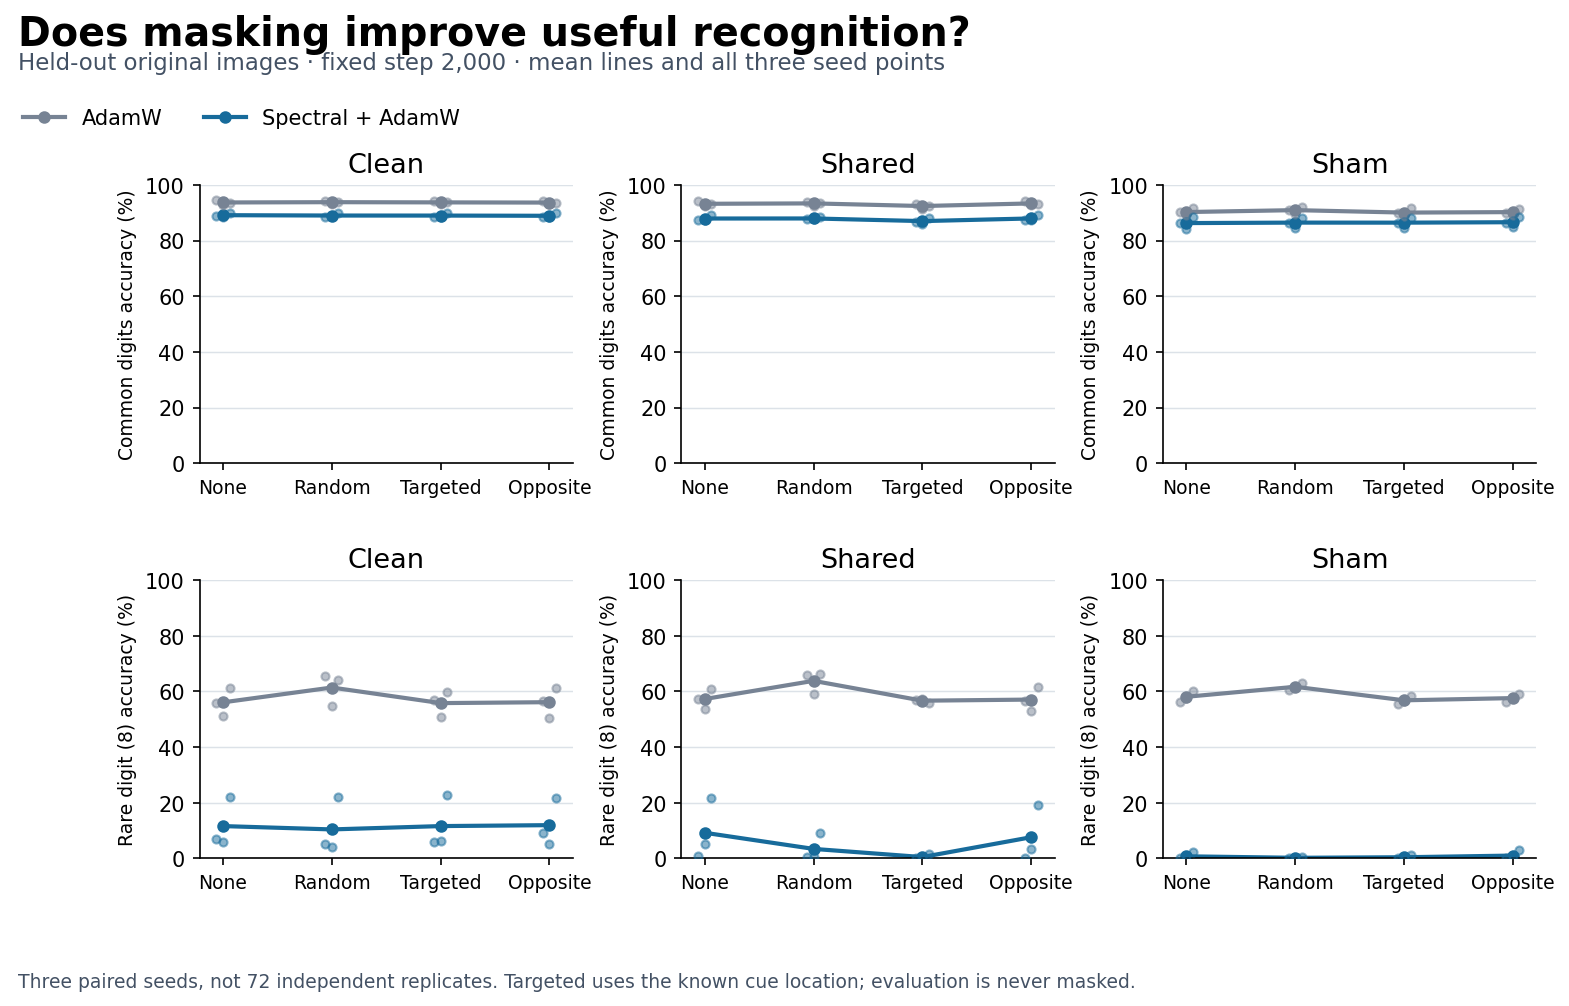
\includegraphics[width=\linewidth]{../../2026-09-10-spectral-augmentation/plots/recognition.png}
\caption{Unpatched common and rare recognition under all mask modes at the fixed endpoint. Small points show three paired seeds; larger markers joined by lines show their means. The direct report separately retains patched-image outcomes, CE, cue components and every preselected learning-curve step. No trajectories were rerun for this figure or appendix.}
\label{fig:augmentation}
\end{figure}

\subsection{Why the cue contrast alone is insufficient}
Using the selectivity study's true-digit definition (digits 1--7 and 9), evaluate 4,000 same-seed held-out images in patched/unpatched pairs. For policy $p$, cell $c$ and mask mode $a$, let
\begin{align}
E_{p,c,a}&=100\left[\Pr(\widehat y_{\rm patched}=0)-\Pr(\widehat y_{\rm unpatched}=0)\right],\\
Q_{p,a}&=E_{p,\mathrm{Shared},a}-E_{p,\mathrm{Sham},a},\\
I_Q(a)&=[Q_{N,a}-Q_{N,\mathrm{None}}]-[Q_{R,a}-Q_{R,\mathrm{None}}].
\end{align}
Here $N/R$ denote native/raw; all quantities are in percentage points and lower is the registered favorable direction. They are not substitutes for the two component error rates. Targeted reduces native Shared $E$ from 95.717 to 92.058 points and $Q$ from 96.275 to 92.775, in every seed. Yet unpatched wrong-0 predictions rise from 1.758\% to 4.025\% in every seed, while patched wrong-0 predictions fall from 97.475\% to 96.083\% in only two seeds. Part of the smaller excess comes from damage to ordinary classification. Raw likewise has a smaller $E$ while its patched wrong-0 rate rises from 99.392\% to 99.800\% in every seed.

For Random, $I_Q$ is favorable in every seed (mean $-1.375$ points) and native $Q$ falls 0.842 points. But native Shared $E$ rises from 95.717 to 95.917 points, while Sham $E$ rises more, from $-0.558$ to $+0.483$. Its Shared patched wrong-0 rate also rises in mean. The favorable interaction therefore does not establish reduced absolute Shared susceptibility. These components are retained rather than relabeling a difference-in-differences as a general robustness gain.

\subsection{A favorable mathematical route with a remaining boundary}
At fixed parameters, total gradient covariance under augmentation decomposes as
\begin{equation}
\Cov(h)=\Cov_i\!\left(\E_a[h\mid i]\right)+\E_i\!\left[\Cov_a(h\mid i)\right].
\end{equation}
Added within-example variation need not increase the total. In a deliberately strong toy model, let a constant additive cue gradient be $Sc$, with $S\sim\mathrm{Bernoulli}(0.1)$. Independent half-erasure gives visibility $V=S(1-A)$ and $\Pr(V=1)=0.05$. Thus
\begin{align}
\E[Sc]&=0.1c,& \Cov(Sc)&=0.09cc^\top,\\
\E[Vc]&=0.05c,& \Cov(Vc)&=0.0475cc^\top.
\end{align}
Independent batch averaging divides these covariances by 64. This supplies a possible route to lower cue prominence, not a measured account of the evolving centered/truncated observer. Real gradient cross-terms, image erasure and optimization dynamics need not follow it. Crucially, the construction still satisfies
\begin{equation}
\Pr(\widetilde y=0\mid\text{surviving inserted Shared cue})=1.
\end{equation}
Erasure reduces cue frequency without making a surviving cue unreliable for its assigned wrong target. This probability concerns the inserted-cue event, not every natural image resembling those pixels. The study constrains this frequency-reduction recipe, not all augmentation or invariant learning. Conversely, static Sham already gives poor native rare recognition, so weakening association alone is not an established remedy. No observer mediation was measured in this study and no additional mask/rank/rate search is selected. The earlier diffuse-corruption preservation and grokking positives remain separate evidence.

\clearpage
\section{Ordinary augmentation: useful learning without a practical spectral gain}\label{app:ordinary-augmentation}
\subsection{Clean and fixed-wrong-label endpoint comparisons}
These studies answer the all-class augmentation question separately from cue masking. Each uses three fresh paired seeds and twelve trajectories: raw AdamW/native stable rank-32 crossed with none/one-view translation. The 50,890-parameter MLP, optimizer and observer settings follow Appendix~\ref{app:methods}, but training now has 500 examples per class and a disjoint balanced 5,000-image held-out set, with every class eligible from update 1. Independent streams fix splits, replacement-sampled occurrences and zero-filled integer shifts $d_x,d_y\in\{-2,\ldots,2\}$. There is no interpolation. Translation starts during the 100-step unfiltered warmup. All trajectories use 4,000 updates of batch 64; original-image logits are retained at 0, 100, 200, 400, \ldots, 4,000. The official test set is unused.

Clean seeds are 202609141--143; wrong-label seeds are 202609151--153. The latter selects exactly 400 of 500 examples per true class and assigns a fixed target uniformly from the other nine classes: 80\% are \emph{actually wrong}, and labels remain attached to each example across all views. These are separate studies, not a paired clean-by-noise factorial. Table~\ref{tab:ordinary-augmentation} gives the fixed endpoint; no best checkpoint is selected.

\begin{table}[htbp]
\centering\small
\begin{tabular}{llrrrr}
\toprule
& & \multicolumn{2}{c}{Clean labels} & \multicolumn{2}{c}{80\% wrong labels}\\
Policy & Translation & Accuracy (\%) & CE & Accuracy (\%) & CE\\\midrule
Raw & None & 92.927 & 0.33046 & 24.653 & 2.39416\\
Raw & Present & 95.653 & 0.15355 & 62.013 & 1.82879\\
Native & None & 87.027 & 0.45716 & 53.007 & 1.97410\\
Native & Present & 82.347 & 0.65677 & 48.640 & 2.11847\\\bottomrule
\end{tabular}
\caption{Three-seed mean original-held-out outcomes at step 4,000. Translation improves raw accuracy and CE and worsens native accuracy and CE in every seed of each study. Sources: \src{output/2026-09-10-spectral-general-augmentation/results.md}{clean report} and \src{output/2026-09-10-spectral-wrong-label-augmentation/results.md}{wrong-label report}, each linked to its independent saved-logit audit and all curves. CE is nats/example; lower is better.}
\label{tab:ordinary-augmentation}
\end{table}

These deficits are not absence of learning. Within each augmentation mode, raw/native model and Adam states match at step 100; the two augmentation modes have different warmups. Clean native accuracy rises 85.687\%$\to$87.027\% without translation and 79.713\%$\to$82.347\% with it. Noisy native rises 46.840\%$\to$53.007\% and 36.947\%$\to$48.640\%, respectively. Native accuracy and CE improve after its own warmup in every seed and mode of both studies. The noisy augmentation accuracy deficit narrows from 9.893 to 4.367 points, but its CE deficit widens from 0.110709 to 0.144370 nats. Useful continued learning therefore coexists with an adverse augmentation endpoint.

Unaugmented native beats unaugmented raw on both noisy primary metrics in every seed. On actually corrupted training examples, its wrong-target accuracy is 7.442\% versus raw's 60.583\%. Yet raw translation reaches 7.842\% while attaining much better true-label competence. Native translation lowers wrong-target accuracy further to 6.358\%, but also lowers wrong-target CE in every seed: assigned-target probability and argmax false-label fit disagree. This is not uniformly less memorization. Raw translation still deteriorates late in held-out accuracy in two seeds while false-label fit rises in all three; its fixed-endpoint advantage is not immunity. The corruption retains population class signal (true-label probability 0.2 versus $4/45$ for each wrong class). Repeated views do not create independent true-label votes.

\subsection{A favorable local direction and a size-only boundary}
The \src{output/2026-09-10-spectral-augmentation-state/results.md}{saved-state diagnostic} reuses only six clean native step-100 parents: three seeds times two warmup modes, not six independent replications. At each fixed parent, 64 training examples and four translated views supply per-example geometry plus five candidate batch gradients (original and four translations). The objectives use original and fixed-translated views of the same 256 held-out examples, disjoint from training. Every raw/native proposal starts from the same private model/Adam state; native observes its candidate once before the single Adam step.

Let $\theta_D$ be the actual rounded FP32 decay endpoint and $d_R,d_N$ the actual raw/native endpoints minus $\theta_D$. Reciprocal controls materialize $\theta_D+d_R\norm{d_N}/\norm{d_R}$ and $\theta_D+d_N\norm{d_R}/\norm{d_N}$, with FP64 norm ratios and checked realized rounding. All controls were available under the fixed zero-norm exclusion and ratio cap 100. The decay-only reference is not Adam with a zero gradient. A second path fraction 0.1 scales the whole displacement, including decay, and is not another optimizer update.

From unaugmented warmups, translated input and translated readout favor the native direction in all three seeds at either matched data-step norm, at both path fractions and in the signed derivative. At raw size, full-step CE-benefit differences are $+0.0000396$, $+0.0001701$, $+0.0000353$ nats. Conversely, translated input with original readout favors raw in every seed under both warmup modes; size matching does not remove that disadvantage. Other cells have mixed or scale-dependent signs. Native data-step norms are 92.53--97.62\% of raw at these first filtered proposals, not collapsed updates. These local findings neither reverse the endpoints nor establish their trajectory mediation.

Under the recorded \emph{pre-update} span, the finite four-view total equals between-image-mean plus within-image-view variation (denominators 64 and $64\times4$). Between retention is 76.93--80.59\%, within retention 34.43--54.21\%, and translated mean-gradient retention 79.05--81.35\%. This preferential retention is real arithmetic, not identification of semantic signal: the finite-view between term still contains view randomness. The native candidate uses its updated basis; gradient-space retention is not Adam utility. Cross-warmup comparisons also change weights and moments, not just observer history.

\subsection{Changing observation while controlling extra views}
Fresh clean seeds 202609161--163 retain the small recipe and translated training throughout. Raw1 delivers the first-view gradient $g_1$ to AdamW. Native1 observes $g_1$ then applies its canonical action. Observer4 observes the sequential FP32 mean $\bar g=(g_1+g_2+g_3+g_4)/4$ once, but delivers the resulting projection of $g_1$ after warmup; it does not ingest $g_1$ again. Raw4 delivers $\bar g$ directly. All four gradients use the same parameters and indexed examples. Raw1/native1/observer4 have identical model/Adam warmups; raw4 already averages during warmup and has a different trajectory. Each policy advances Adam once per update.

\begin{table}[htbp]
\centering\small
\begin{tabular}{lrrrr}
\toprule
& \multicolumn{2}{c}{Original heldout (primary)} & \multicolumn{2}{c}{Translated heldout (secondary)}\\
Policy & Accuracy (\%) & CE & Accuracy (\%) & CE\\\midrule
Raw1 & 95.173 & 0.156650 & 93.527 & 0.220596\\
Native1 & 81.393 & 0.660327 & 67.073 & 1.040954\\
Observer4 & 81.593 & 0.660356 & 68.687 & 1.020062\\
Raw4 & 95.633 & 0.144492 & 94.207 & 0.198985\\\bottomrule
\end{tabular}
\caption{Fresh three-seed four-arm means at update 4,000. Every arm has the same underlying occurrence count, but four-view arms use four times the batch-gradient evaluations. Sources: \src{output/2026-09-10-spectral-multiview-clean/results.md}{multiview report}, with all paired contrasts, warmup values and 22-state curves, and its independent saved-logit audit. No cross-study pooling or selected epoch is used.}
\label{tab:multiview}
\end{table}

Observer4 improves translated held-out accuracy over native1 by 1.88/1.44/1.52 points and CE by 0.027265/0.015959/0.019452 nats. Both metrics also improve from observer4's own warmup in every seed: this secondary positive includes useful learning, not just better covariance capture. Original accuracy differences are $+0.16/+0.70/-0.26$ points; original CE improves in one seed and worsens in two. Its near-zero mean CE contrast is cancellation, not equivalence. Both spectral policies improve original accuracy and CE from warmup in every seed; native1's translated accuracy nevertheless falls in two seeds despite improving CE.

Raw4 beats raw1 on both readouts and metrics in every seed, and both raw policies beat both spectral policies in all those comparisons (Table~\ref{tab:multiview}). Observer4's original training accuracy is also only 82.38\%, versus raw4's 97.667\%: the weak held-out result is not a generalization gain hidden by excessive training fit. Four-view trajectories require 16,000 batch-gradient evaluations versus 4,000; the twelve arms total 120,000. This controls view count against raw4, not wall time. Self-inclusion of $g_1$ in $\bar g$, changed observation magnitude and diverging learning/observer histories remain intertwined; the policy comparison does not isolate population covariance variance. No noisy-label four-view result establishes retained protection.

\newpage
\subsection{Historical fairness and the larger-configuration bridge}
The small-model result does not erase the stronger unaugmented regime. Historical legacy rank-200 endpoints at seeds 42/43/44 are 74.28/81.87/83.06\% versus Adam's 35.92/37.74/38.00\%. A later matched stable-hard AdamW comparison retains a positive at seed 42: global rank 200 reaches 78.77\% versus raw 38.93\%. This stable positive is single-seed; the per-matrix rank-64 endpoint of 81.74\% followed selection on the same seed's test performance. Legacy seed 42 falls from 86.00\% peak to 74.28\% endpoint, and historical raw early test peaks are not deployable validation-stopping results. These qualifications accompany, rather than dismiss, the useful late-horizon protection.

That regime uses 235,146 parameters, standardized pixels, all 60,000 training examples and roughly 56,280 updates over 60 shuffled passes. Its 90\% uniform replacement implies about 81\% actually wrong labels in expectation, close to the new 80\%, not a ten-point severity difference. Rank, model, normalization, exposure and readout all change; neither rank alone nor rank/parameter ratio explains the contrast, and absolute cross-study accuracies cannot be ranked as matched outcomes. No cited historical strong-regime result tests ordinary translation. See the \src{research/noisy_mnist_hard_curves.md}{stable historical report} and \src{output/2026-09-10-spectral-multiview-clean/regime-comparison.md}{cross-regime evidence review}.

The subsequently completed bridge tests the larger stable configuration directly, preserving the favorable unaugmented comparison without inferring an augmentation benefit from it. Its new internal validation/reporting split changes historical data roles and repetition. Equal total example exposure does not make it an exact reproduction, nor does a comparison across several changed settings isolate rank as the explanation. The fixed \src{output/2026-09-10-spectral-strong-augmentation/protocol.md}{protocol} and \src{output/2026-09-10-spectral-strong-augmentation/results.md}{completed report} remain authoritative.

\newpage
\subsection{Strong rank-200 filtering learns, but adds no translation benefit}\label{app:strong-augmentation}
Three fresh paired seeds (202609171--173) cross raw AdamW/native stable rank-200 with none/translation: twelve trajectories. The 784--256--128--10 ReLU MLP has 235,146 parameters. Each seed randomly partitions the official training set into 50,000 training, 5,000 clean validation and 5,000 clean reporting images; roles are disjoint within seed, not across seeds. Ninety-percent uniform replacement gives 80.962/81.016/81.012\% actually wrong labels, fixed across all views and passes. Translations remain zero-filled integer shifts in $[-2,2]$, applied before standardization by $(x-0.1307)/0.3081$; every evaluation uses original images.

AdamW and the unchanged canonical stable hard observer use the historical learning rate 0.001, weight decay 0.01, decay 0.99 and 100-update unfiltered warmup, without moment reset or gain restoration. Raw/native model and Adam warmups agree within augmentation mode. Each arm takes 72 shuffled full passes: 3.6 million example exposures, 56,304 updates including each final 16-example batch. This matches historical exposure, not its 56,280-update trajectory. The 74 readouts are initialization, update 100 and every epoch endpoint. All twelve minimum-validation-CE choices were persisted and verified before reporting arithmetic, using the fixed FP64 reduction and earliest exact tie. Both selected metrics use that one checkpoint, not separate best epochs.

\begin{table}[!ht]
\centering\small
\begin{tabular}{llrrrr}\toprule
& & \multicolumn{2}{c}{Fixed final} & \multicolumn{2}{c}{Validation-CE selected}\\
Policy & Translation & Accuracy (\%) & CE & Accuracy (\%) & CE\\\midrule
Raw & None & 32.000 & 2.708446 & 72.487 & 1.757167\\
Native200 & None & 79.753 & 1.854416 & 82.973 & 1.808122\\
Raw & Present & 84.973 & 1.804289 & 85.993 & 1.764379\\
Native200 & Present & 66.820 & 1.981758 & 68.673 & 1.931696\\\bottomrule
\end{tabular}
\caption{Strong-bridge clean reporting means across three paired seeds. CE is nats/example, lower better. The primary is native200 versus raw \emph{with translation} at the fixed final endpoint; selected checkpoints are secondary and require clean validation data. All seeds, stopping exposures and late-window values are in the \src{output/2026-09-10-spectral-strong-augmentation/results.md}{direct report} and \src{output/2026-09-10-spectral-strong-augmentation/audit.json}{independent saved-array audit}.}
\label{tab:strong-augmentation}
\end{table}

The constructive result is substantial continued learning. Unaugmented native rises from 36.700\% at warmup to 79.753\%, gaining 35.08/38.68/55.40 points (mean 43.053); CE falls in every seed, mean 0.284756 nats. Its final advantage over unaugmented raw is 44.16/49.30/49.80 points, with lower CE in every seed. At own validation-selected checkpoints it still wins accuracy in all seeds (mean 10.487 points), but \emph{loses CE in every seed} (mean excess 0.050955). This is not general dominance over legitimate stopping. Translated native also learns: 26.120\%$\to$66.820\%, a 40.700-point gain, with CE improvement in every seed. Neither policy merely freezes its warmup.

The augmented primary is nevertheless adverse in all three seeds: native-minus-raw accuracy is $-20.44/-19.18/-14.84$ points (mean $-18.153$); native CE is higher by $0.181014/0.151446/0.199948$ nats. Validation-selected and epoch-61--72 late-mean comparisons also lose every seed and both metrics, with mean accuracy deficits 17.320/19.708 points and CE excesses 0.167317/0.185124. Translation itself helps raw and hurts native at the fixed endpoint in every seed and both metrics; the accuracy interaction is $-65.907$ points. Raw translation also beats unaugmented native at final and selected reporting. Raw augmentation's selected CE, however, is worse in two seeds and slightly worse in mean than selected raw without augmentation. No selected-metric blanket win is asserted.

\newpage
\begin{figure}[!ht]
\centering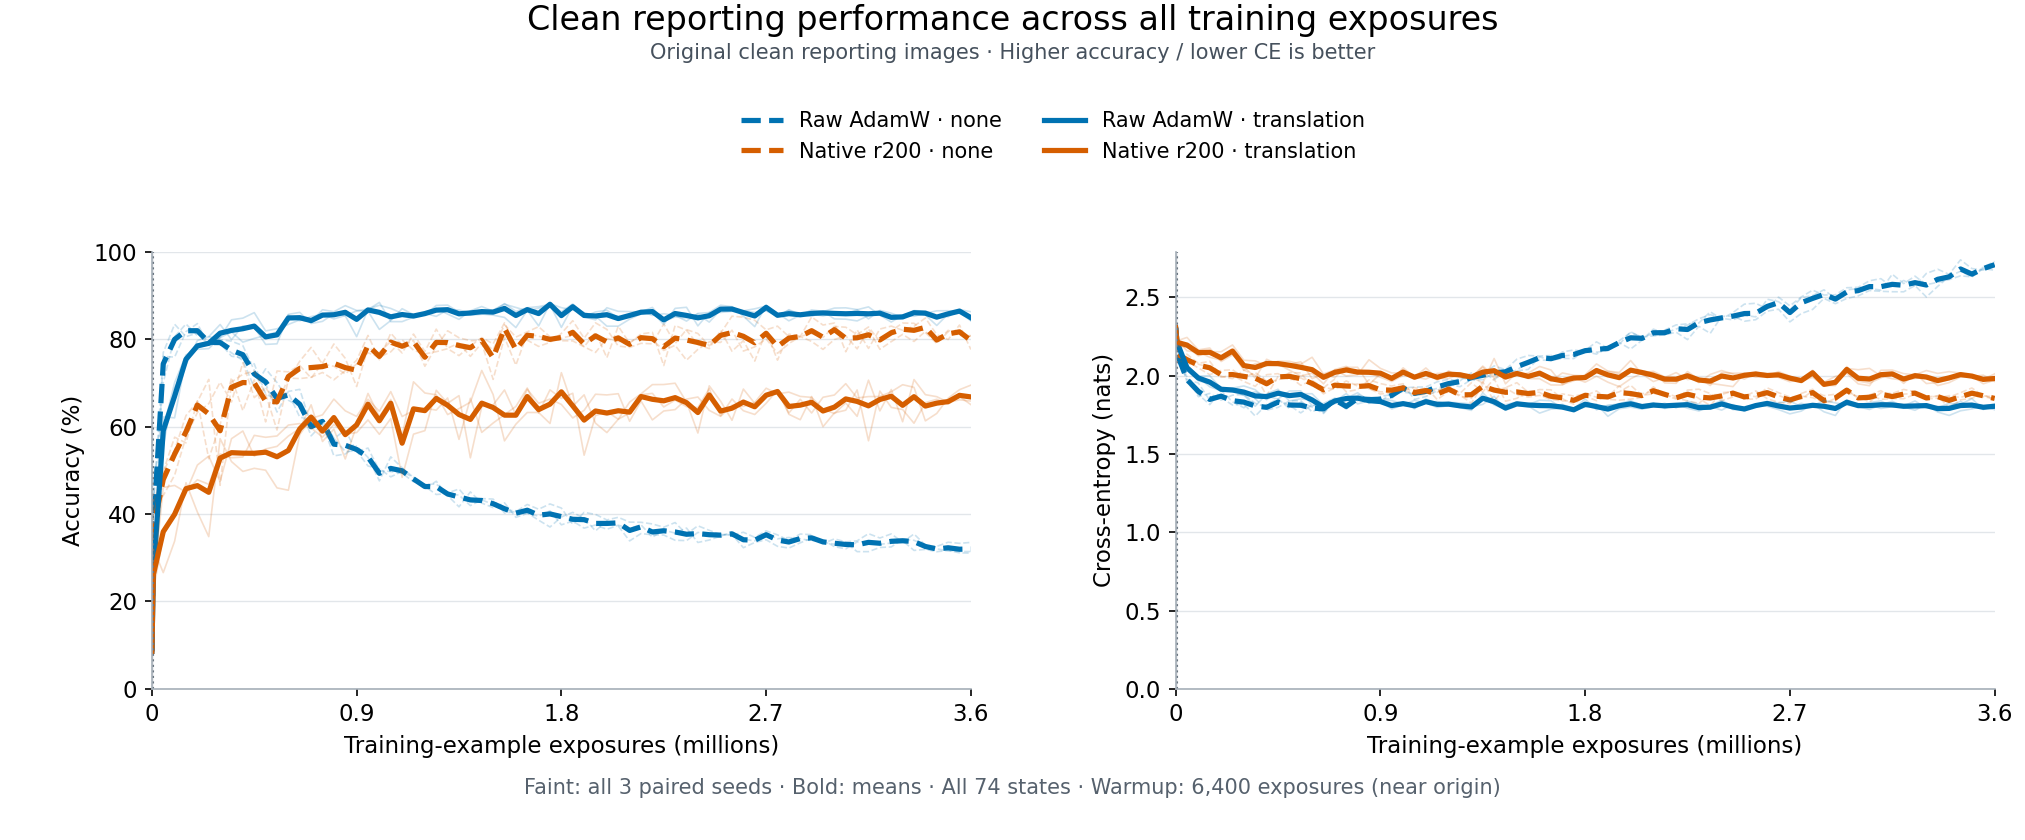
\includegraphics[width=\linewidth]{../../2026-09-10-spectral-strong-augmentation/reporting-learning-curves.png}
\caption{Completed strong-bridge reporting curves, reused unchanged. Faint lines show all three paired seeds and bold lines their means across all 74 fixed states. The unaugmented raw early peak and later deterioration remain visible beside useful native learning and the adverse combined recipe. The same 3.6 million example exposures are used per arm; this is not a matched-time comparison.}
\label{fig:strong-augmentation}
\end{figure}

The training-label components constrain the explanation. On actually wrong examples, final assigned-label accuracy/CE are 39.158\%/1.649918 for raw/none, 2.517\%/2.376372 for native/none, 2.230\%/2.377909 for raw/translation and 3.762\%/2.355321 for native/translation. Both single interventions restrict wrong-assignment fit relative to raw/none while supporting clean prediction. Combining them gives \emph{more} such fit than either single intervention in every seed: higher wrong-target accuracy and lower wrong-target CE. Lower all-training assigned accuracy is not extra noise suppression when useful fitting of correctly assigned examples also falls. These are original-image fit proxies, not identified memorization circuitry.

The independent NumPy audit passes 937 artifact checks and 888 saved-logit states, verifies all twelve validation choices before reporting, and finds maximum scalar discrepancy $1.46\times10^{-11}$ within fixed $10^{-10}$ tolerances. Its two logit passes respect the memory cap. Checkpoint bytes are hashed without deserialization; model/Adam digests remain producer assertions checked for pairing, not independently reconstructed states. Reporting arrays were saved but not cryptographically blinded. A separate \src{output/2026-09-10-spectral-strong-augmentation/interpretation-review.md}{scalar and interpretation review} corroborates all registered windows without rerunning neural computation.

Each arm has the same gradient count. Mean branch wall times are 254.424, 695.874, 272.787 and 728.823 seconds in Table~\ref{tab:strong-augmentation} order. These are implementation costs, not optimized speed or time-to-target claims. Three paired seeds on an adaptively revisited MNIST task do not establish transfer or safety efficacy. The bridge shows that small rank 32 is not a sufficient explanation for the earlier adverse augmentation result; it does not identify which update components or Adam-history effects cause the larger configuration's deficit. Conditional mathematical complementarity remains possible, not experimentally demonstrated here. No acquisition, audit or scientific tensor analysis was rerun for this integration, and no further experiment is selected by it.

\clearpage
\section{Conditional objective and feature geometry}\label{app:conditional-geometry}
Two reviewed calculations sharpen the constructive account without adding neural evidence. Augmentation changes the objective through both a combined prediction and view consistency; random-label gradients can reveal feature geometry even when their mean class signal is weak. Their connection is conditional: useful restriction requires the retained geometry to support the desired signed update. The identities below specialize established algebra, not novel theorems or an identified mechanism for the completed comparisons in Appendix~\ref{app:ordinary-augmentation}.

\subsection{What augmentation optimizes, and what retained energy does not imply}
Fix an image $x$, parameters $\theta$ and a probability target $t$ common to all views. Let $T$ have finite support with fixed probabilities independent of $\theta$. With $K$ logits, define
\begin{equation}
z_T=f_\theta(Tx),\quad \bar z=\E_Tz_T,\quad
A(z)=\log\sum_{k=1}^K e^{z_k},\quad
\ell(z,t)=A(z)-t^\top z.
\end{equation}
For $p_T=\operatorname{softmax}(z_T)$ and $\bar p=\operatorname{softmax}(\bar z)$, linearity of the target term and convexity of $A$ give exactly
\begin{align}
\E_T\ell(z_T,t)&=\ell(\bar z,t)+R,\qquad R=\E_TA(z_T)-A(\bar z)\geq0,\label{eq:view-objective}\\
R&=\E_T\operatorname{KL}(\bar p\Vert p_T),\qquad
\bar p_k=\frac{\exp(\E_T\log p_{T,k})}{\sum_j\exp(\E_T\log p_{T,j})}.\label{eq:view-kl}
\end{align}
The center is the normalized geometric mean, not generally $\E_Tp_T$; the KL center is the first argument. Averaging $\operatorname{KL}(\bar p\Vert p_T)=A(z_T)-A(\bar z)-\bar p^\top(z_T-\bar z)$ proves the second identity. This is not Jensen--Shannon divergence. Nor need $\bar z=f_\theta(x)$: the exact decomposition is not original-image loss plus the same penalty. At finite logits, $R=0$ precisely when all positive-probability views have identical class probabilities, allowing class-independent logit shifts. No internal-representation invariance follows.

Label-independent log-partition regularization has direct precedents in feature noising \citep[\S2, Eqs.~4--6]{wager2013dropout} and augmentation's averaging/variance analysis \citep[\S\S4.1--4.2]{dao2019augmentation}. The geometric-center CE decomposition is explicit in \citet[Appendix B.3, Eqs.~32--33]{wood2023diversity}, crediting Heskes; substituting augmentation views is an application, not a priority claim.

For example $i$, let $q_i$ be its corruption-law expected target and $\epsilon_i=t_i-q_i$ its fixed realized assignment residual. Then
\begin{align}
L_{\rm fixed,aug}&=S+F+C,\\
S&=\frac1N\sum_i\ell(\bar z_i,q_i),\quad
F=-\frac1N\sum_i\epsilon_i^\top\bar z_i,\quad
C=\frac1N\sum_iR_i.
\end{align}
These are soft-target fitting, fixed-assignment force and view disagreement, not pure semantic components. In ten-class 90\% uniform replacement, $q=0.1e_y+0.9u$ with $u_k=0.1$: $q_y=0.19$, others $0.09$, and 81\% actually wrong in expectation. This differs from exactly 80\% guaranteed wrong. At independently fixed $\theta$, $\E_\epsilon F(\theta)=0$; that cannot be applied to parameters fitted to those same assignments. $C$ is label-independent only at the same model/images/view law. A consistently wrong predictor can have $C=0$; repeated views retain the same wrong label, not independent truth votes.

At differentiable logits, write $J_T=\partial z_T/\partial\theta$ and $\bar J=\E_TJ_T$. For one example, the exact gradient split is
\begin{equation}
\nabla\ell_{\rm aug}
=\underbrace{\bar J^\top(\bar p-q)}_s
+\underbrace{(-\bar J^\top\epsilon)}_f
+\underbrace{\E_T[J_T^\top(p_T-\bar p)]}_c.
\label{eq:view-gradient}
\end{equation}
The moving center is differentiated, not a stop-gradient teacher. Averaging view-loss gradients estimates all three terms; differentiating only mean-logit loss omits $c$. The consistency gradient is a mean involving Jacobians and predictions, not a within-view gradient covariance component.

For a frozen orthoprojector $P$, total gradient $g$ and $r_C=\nabla C$, plain projected descent gives $\Delta C=-\eta r_C^\top Pg+o(\eta)$, not $-\eta\norm{Pr_C}^2$. The example $r_C=(1,0.1)^\top$, $g=(-1,20)^\top$, $P=\operatorname{diag}(1,0)$ has retention $100/101$, yet $r_C^\top g=1$ and $r_C^\top Pg=-1$. Raw decreases $C$ locally while projection increases it; both decrease the total loss. The \src{output/2026-09-10-spectral-augmentation-theory/independent-math-review.md}{independent derivation} realizes these vectors by two affine binary-logit views. Exact full retention $Pr_C=r_C$ is the special boundary that preserves this signed utility. For actual Adam displacement the relevant first-order change is $r_C^\top\Delta\theta$, with finite-step checks, not the projected-GD expression.

\subsection{When gradient covariance is exactly feature second-moment geometry}
Now freeze a feature map $h(x)\in\R^d$ and evaluate a fixed last layer $W\in\R^{K\times d}$, $K\geq2$, with logits $Wh$ and finite $M=\E[hh^\top]$. For column-major vectorization of its CE matrix gradient,
\begin{equation}
G=(p-e_Y)h^\top,\qquad g=\operatorname{vec}(G)=h\otimes(p-e_Y).
\end{equation}
Assume $p=u=\mathbf1/K$ on the input support and fresh uniform labels $Y$ independent of $h$. With $\Pi_c=I-\mathbf1\mathbf1^\top/K$, the conditional label residual has mean zero and covariance $\Pi_c/K$, hence
\begin{equation}
\E g=0,\qquad \Cov(g)=M\otimes(\Pi_c/K).\label{eq:feature-covariance}
\end{equation}
Here $M$ is the \emph{uncentered second moment}, not $\Cov(h)$: even a constant feature produces gradient variation. This is an exact special case of familiar activation/error Kronecker algebra \citep[\S\S1.2--2]{martens2015kfac}. Hard truncation is not K-FAC's inverse preconditioning. Uniform labels equal model-sampled labels at $p=u$, so this special covariance also equals the last-layer Fisher and affine-logit CE Hessian; observed-label second moments, centered covariance and Fisher differ generally \citep[\S\S2, 4--5]{kunstner2019empirical}.

If $Mv_j=\lambda_jv_j$, each positive feature eigenvalue contributes $K-1$ eigenvalues $\lambda_j/K$, with eigenvectors $v_j\otimes a$ for unit class contrasts $a\perp\mathbf1$. For $r<d$ and a strict gap $\lambda_r>\lambda_{r+1}$, let $V_r=[v_1,\ldots,v_r]$. The leading rank $r(K-1)$ action is
\begin{equation}
P_r=(V_rV_r^\top)\otimes\Pi_c,\qquad
P_r\operatorname{vec}(G)=\operatorname{vec}(GV_rV_r^\top).\label{eq:feature-projection}
\end{equation}
The last identity uses $\Pi_cG=G$, since gradient columns sum to zero. Class-contrast copies are degenerate, not identified semantic clusters. Cutting through such a block or a feature tie need not yield a unique feature-only projector. Feature scaling changes $M$ quadratically; high energy is not a representation-invariant importance ranking. A population gap also does not guarantee accurate finite-history estimation.

\newpage
\subsection{Partial corruption: a constructive retention case and its boundary}
At $p=u$, replace the true label by a fresh uniform label with probability $\rho$, otherwise retaining it. Define $g_c=h\otimes(u-e_y)$, $\mu_c=\E g_c$, $S_c=\E[g_cg_c^\top]$ and $S_u=M\otimes(\Pi_c/K)$. Mixture conditioning gives
\begin{equation}
\E g=(1-\rho)\mu_c,\qquad
\Cov(g)=\rho S_u+(1-\rho)S_c-(1-\rho)^2\mu_c\mu_c^\top.\label{eq:mixed-feature-covariance}
\end{equation}
$S_c,S_u$ are second moments; omitting the mean subtraction changes the spectral object. For a binary example take $W=0$, independent balanced signs $s,n\in\{-1,1\}$ and $h=(as,bn)^\top$, $a,b>0$, with truth determined by $s$. The second feature is independent nuisance. The expected class gradient lies entirely in feature 1, while the two class-contrast covariance eigenvalues are
\begin{equation}
\lambda_{\rm signal}=\frac{a^2\rho(2-\rho)}2,\qquad
\lambda_{\rm nuisance}=\frac{b^2}2.
\end{equation}

\begin{table}[!ht]
\centering\small
\begin{tabular}{llrrr}\toprule
Amplitudes & Leading direction & Mean retained & Variance before & Variance after\\\midrule
$a=2,b=1$ & Signal & 100\% & 2.48 & 1.98\\
$a=1,b=2$ & Nuisance & 0\% & 2.495 & 2.00\\\bottomrule
\end{tabular}
\caption{Analytic binary examples at $\rho=0.9$, retaining the leading rank-one direction. Variance is $\operatorname{tr}\Cov(g)$, not loss or accuracy. These are exact algebraic cases, not observed training outcomes.}
\label{tab:feature-geometry}
\end{table}

The favorable case preserves the entire expected noisy-objective gradient and clean-signal direction while removing independent nuisance variance: an unbiased lower-variance estimate of that fixed objective's gradient. The identical rule under reversed feature scales discards all nonzero mean class signal. At $\rho=0$, this construction's consistent signal has zero centered variance; at $\rho=1$, geometry remains but expected supervised class signal vanishes. Random labels do not supply the missing mapping to true class names.

These observations make complementarity possible, not established. Augmentation can penalize view-specific fitting while leaving transformation-consistent memorization available. An appropriately aligned learned filter could further restrict that fitting while retaining shared-class and consistency learning; an adverse filter can block those same useful adjustments. Low-rank/diffuse-Jacobian robustness has a direct constructive precedent \citep[Theorems 2.2 and 4.1]{li2020earlystopping}, but its squared-loss and restricted-corruption assumptions do not prove this multiclass-CE method or a 90\%-replacement guarantee.

The gap to the actual optimizer remains material. With fresh uniform labels, nonuniform predictions add $\Cov(h\otimes(p-u))$ to Equation~\eqref{eq:feature-covariance}; this is not a universal additive correction under partial corruption or fixed labels. Fixed reused labels entangle assignments with learned features. Full-network gradients have Jacobian and cross-layer structure, not generally Equation~\eqref{eq:feature-covariance}. Independent fresh batch means scale covariance by $1/B$; dependence and ordering can change it. Temporal centering, drift, forgetting, truncation, current-input self-inclusion and subsequent Adam further separate native training from these fixed-state matrices. Neither a consistency score nor retained variance establishes useful signed motion or neural mediation. The completed small- and strong-recipe results do not identify these components' trajectory roles. No new measurement or diagnostic is selected by this appendix.

\clearpage
\subsection{Signed component utility at reused strong-bridge states}\label{app:component-utility}
The completed \src{output/2026-09-10-spectral-component-utility/results.md}{common-state diagnostic} tests a specific local explanation: does filtering remove consistency learning that raw AdamW would usefully perform? It reuses twelve native rank-200 states from Appendix~\ref{app:strong-augmentation}: three seeds (202609171--173), prior training without/with translation, and steps 100/56,304. These are outcome-informed states on a reused task, not twelve fresh replications. At each parent, two disjoint fixed 64-example action batches receive fixed sampled translations. Every action is translated, including at an unaugmented parent, where it represents hypothetical augmentation onset rather than its actual next training input.

Each paired action starts from the same parameters, inherited Adam moments and observer. Raw bypasses the observer; native observes the identical assigned-CE gradient once, filters it and advances Adam once. Private endpoints are discarded, not continued. A disjoint-from-action 256-example training evaluation panel $I$ supplies the exact uniform grid of 25 shifts in $\{-2,-1,0,1,2\}^2$; a separate 128-example reporting panel supplies clean readouts. Panels and the two action draws are fixed within seed and reused across its four parents. No evaluation-component gradient is supplied as an action.

On $I$, use the preceding exact $L=S+F+C$ split with $q_i=0.1e_{y_i}+0.9u$, differentiating mean logits without a detached teacher. $H_O$ is original reporting true-label CE; $H_T$ is mean per-view reporting CE, not CE of mean logits. Full points preserve actual endpoint bytes: $\theta_{a,1}=\theta_a$. The tenth point is $\theta+0.1(\theta_a-\theta)$ with subtraction, multiplication and addition each executed separately in FP32, not exact arithmetic followed by one rounding. The estimands are
\begin{align}
E_J(a,\alpha)&=J(\theta)-J(\theta_{a,\alpha}),\qquad
U_J(a,\alpha)=-\nabla J(\theta)^\top(\theta_{a,\alpha}-\theta),\\
D_J(\alpha)&=E_J(\mathrm{native},\alpha)-E_J(\mathrm{raw},\alpha).
\end{align}
Derivative displacements subtract after FP64 casting of the actual rounded points. Positive means a decrease of the named objective, not automatically useful learning. The tenth path is a geometric check, not a lower-learning-rate Adam step or one tenth of the measured full effect. Same-fraction rounded decay-only references accompany both policies; this is not zero-gradient Adam. Two draws, three endpoints (raw/native/decay) and two fractions give 144 endpoint readouts across the twelve parents.

\begin{table}[!ht]
\centering\footnotesize
\setlength{\tabcolsep}{3pt}
\begin{tabular}{lrrrrrrr}\toprule
& & \multicolumn{3}{c}{$H_O$ decrease} & \multicolumn{3}{c}{$C$ decrease}\\
Seed & Path & Raw & Native & $D_{H_O}$ & Raw & Native & $D_C$\\\midrule
171 & $1$ & $-546.351894$ & $-539.756434$ & $+6.595461$ & $-9.977187$ & $-10.020139$ & $-0.042952$\\
172 & $1$ & $+1823.412024$ & $+1811.514656$ & $-11.897367$ & $-79.503848$ & $-79.353080$ & $+0.150767$\\
173 & $1$ & $+5608.213952$ & $+5599.399109$ & $-8.814843$ & $-126.967806$ & $-126.571498$ & $+0.396308$\\\midrule
171 & $0.1$ & $-43.771899$ & $-43.225785$ & $+0.546114$ & $-0.328408$ & $-0.334026$ & $-0.005619^{*}$\\
172 & $0.1$ & $+193.343685$ & $+192.170092$ & $-1.173593$ & $-7.299164$ & $-7.284541$ & $+0.014623$\\
173 & $0.1$ & $+558.383293$ & $+557.526631$ & $-0.856662$ & $-10.976195$ & $-10.941365$ & $+0.034831$\\\bottomrule
\end{tabular}
\caption{All three translated-final parents; full paths are primary and actual tenth paths secondary. Values are micro-nats ($10^{-6}$ nats), averaging two draws within each parent; seed suffixes denote 202609171--173. Raw and native $C$ decreases are negative in every row: both worsen consistency. $^{*}$ marks an absolute finite contrast $\leq10^{-8}$ nats, not a zero or an equivalence margin. Direct full-precision scalars: \src{output/2026-09-10-spectral-component-utility/audit.json}{independent audit}; complete reductions and per-draw qualifications: \src{output/2026-09-10-spectral-component-utility/interpretation-analysis.md}{interpretation}.}
\label{tab:component-utility}
\end{table}

The primary clean contrast is favorable in seed 171 and adverse in 172/173, only $(+6.60,-11.90,-8.81)\times10^{-6}$ nats. Seed 171 suffers less clean damage; the others make slightly less positive clean progress. Raw itself worsens $C$ in all three seed averages, including its linear readout. In the two clean-adverse seeds, native actually attenuates that consistency deterioration. Thus this test does not support \emph{lost useful raw consistency learning} at the registered translated-final states. It does not establish no filter effect. Both draws agree on each primary clean-contrast sign, but seed 172's full $C$ contrasts are $-2.13172\times10^{-7}$ and $+5.14707\times10^{-7}$ nats: a positive mean is not an all-draw ordering.

\newpage
\begin{figure}[!ht]
\centering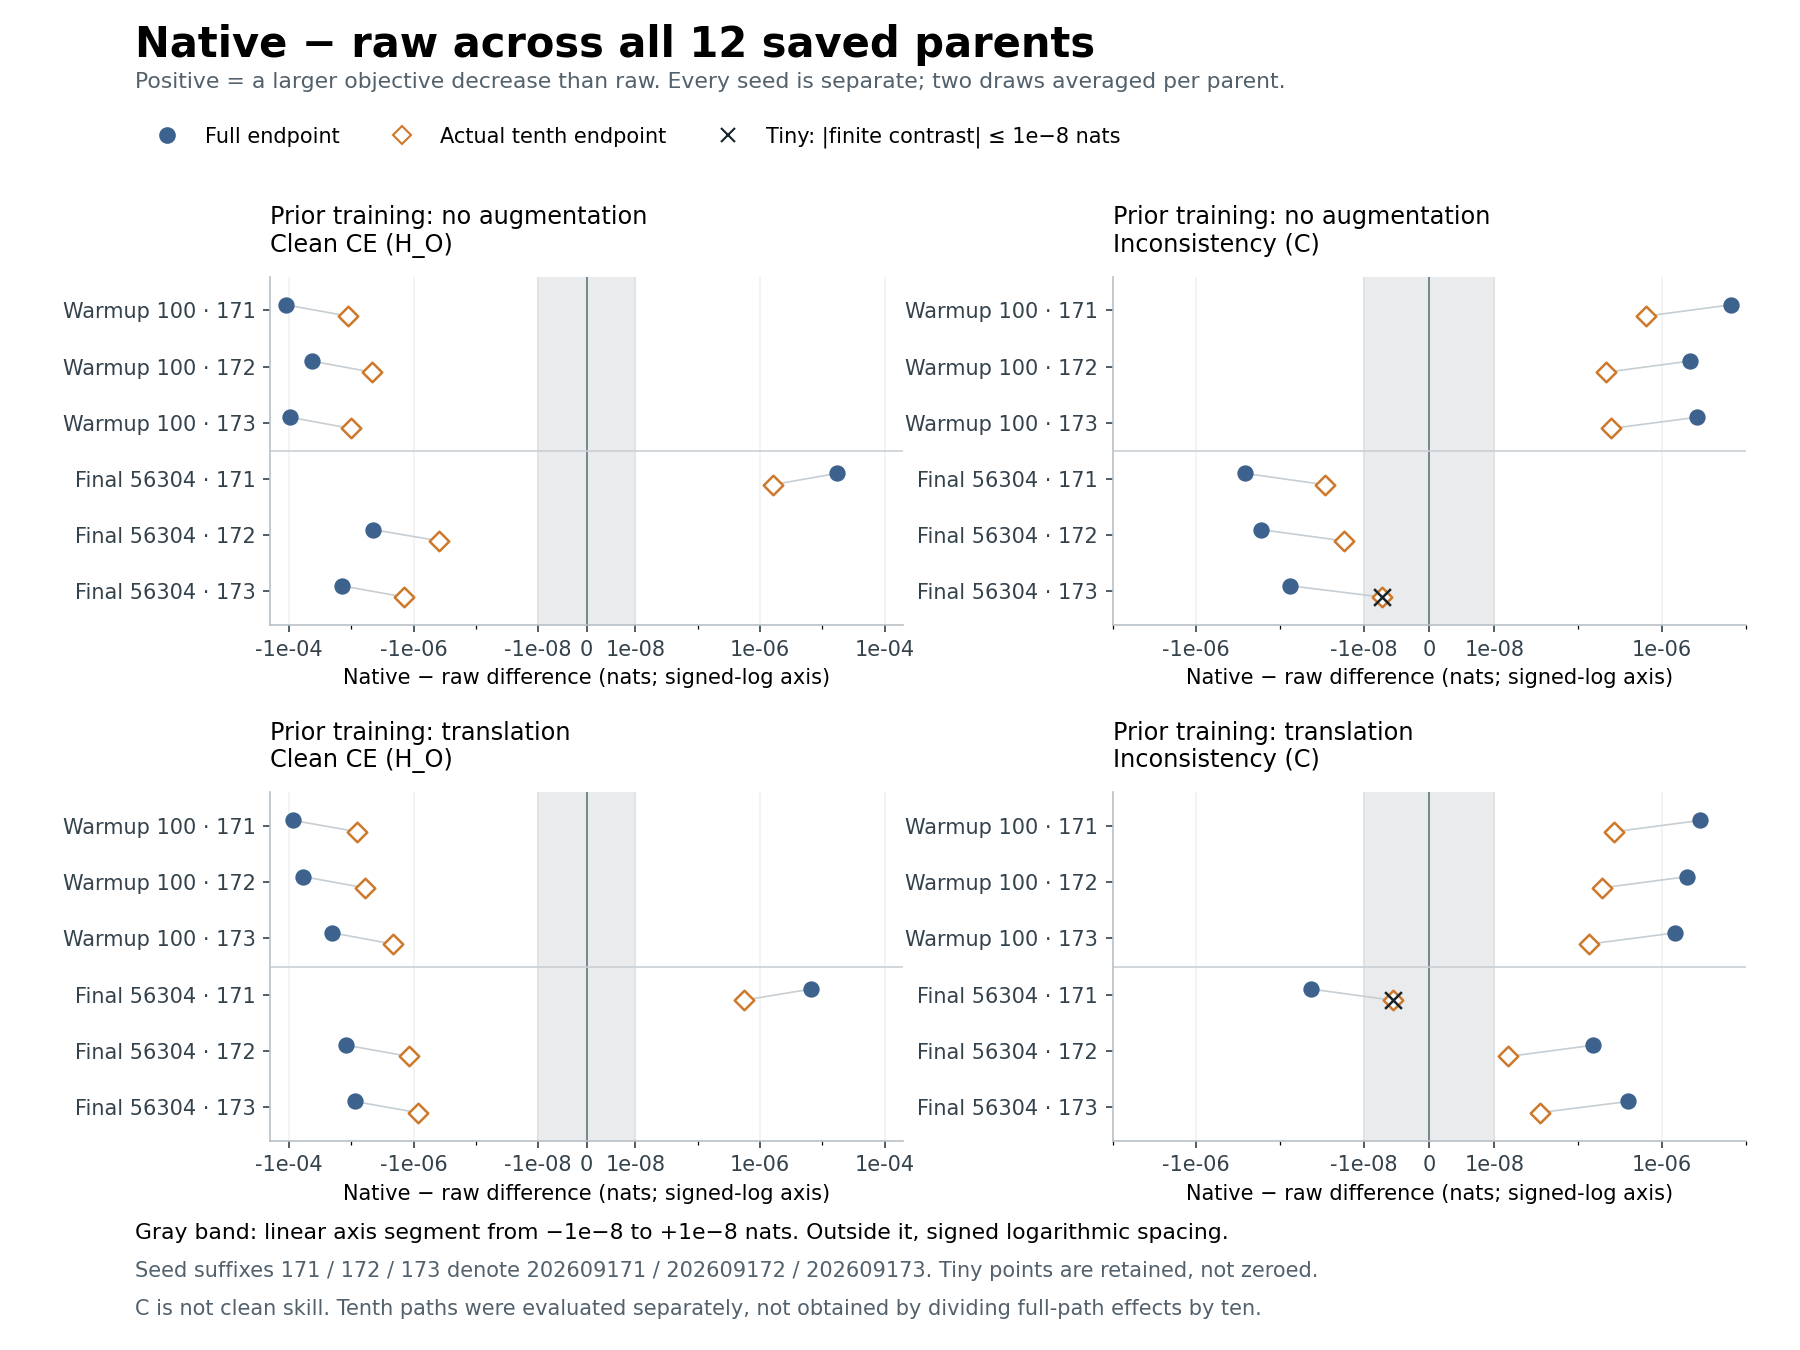
\includegraphics[width=.95\linewidth]{../../2026-09-10-spectral-component-utility/all-parent-contrasts.png}
\caption{All twelve parents and both actual path sizes; existing plot unchanged. Segments pair endpoints, not measured intermediate trajectories. Crosses flag tiny contrasts; axes are signed logarithmic outside the shaded linear $\pm10^{-8}$-nat region. Positive means relatively more decrease, not necessarily absolute progress. Lower $C$ is not clean skill. The \src{output/2026-09-10-spectral-component-utility/plots-manifest.json}{manifest} binds every value to the audit.}
\label{fig:component-utility}
\end{figure}

\paragraph{Secondary cells and actual wrong-label fitting.}
At warmup, native improves relative $C$ while worsening $H_O/H_T$ in all three seeds under both prior-training modes and path sizes. Relative consistency improvement can mean less deterioration. Original/per-view wrong-subset CE also moves relatively toward assigned wrong targets and away from true targets; some cases are less \emph{unfitting}, not absolute wrong fitting. These are six related parents, not independent seeds. Unaugmented final clean effects are mixed while $D_C<0$ in every seed average; this secondary cell does not replace the primary.

$F$ is not wrong-subset fit: primary full-step $D_F>0$ in all seeds, but original wrong-target CE contrasts are $-2.011719,+2.686962,+0.808132$ micro-nats. Seed 171 has less wrong fitting despite its $F$ advantage; the others have less unfitting. Original wrong-target and clean-reporting accuracies are unchanged, not equivalent by inference. Primary $D_L>0$ likewise means less deterioration, not absolute assigned-loss progress. $S=0.1S_{\rm true}+0.9S_{\rm uniform}$ can conceal opposing terms and is not clean CE.

\paragraph{Scope of the numerical and mechanistic statements.}
The independent saved-array audit passes 50,388 checks covering provenance/panels, objectives/dots, rounded paths, Adam algebra and post-basis projection; it does not replay model/autograd or full observer history. This integration reruns neither science nor audit. Magnitudes $\leq10^{-8}$ nats (finite effects/contrasts) or $\leq10^{-10}$ (linear utilities) are small-effect guards, not directional evidence or equivalence margins. Absolute effects can differ appreciably from their derivatives even when paired contrasts agree closely; smaller-path checks do not certify exact linearity.

Common decay cancels in paired contrasts, not absolute effects. Native motion is not uniformly smaller; no norm-matched control isolates direction from magnitude. These actions establish neither trajectory mediation nor alternative-filter efficacy. Earlier useful native learning without augmentation (36.70\%$\to$79.75\%) and its adverse translated endpoint (66.82\% versus raw's 84.97\%) remain intact. Small local differences do not rule out accumulated state/history effects or explain that gap.

\clearpage
\section{Evidence and figure source map}\label{app:sources}
Each entry starts with a repository-relative path; subsequent short paths are relative to that entry's named study directory. The compiled paper includes existing figures unchanged; their underlying reports, registered protocols and raw-linked summaries remain authoritative.
{\small
\begin{description}
\item[Argument and exact methods.] \path{research/spectral_paper_core_2026-09-10.md}; \path{research/spectral_paper_methods_2026-09-10.md}; broader ledger \path{research/spectral_paper_draft_2026-09-09.md}.
\item[Safety framing.] \path{research/spectral_safety_contribution_2026-09-10.md}; targeted primary-source and independent framing check in \path{output/2026-09-10-spectral-safety-framing/source-review.md}. This is writing/attribution, not an additional behavioral safety study.
\item[Selective-continuation derivation.] \path{output/2026-09-06-spectral-optimizer-investigation/analysis/steelman-selective-learning.md}.
\item[Selectivity and Figure 1.] \path{output/2026-09-09-spectral-selectivity-boundary/results.md}; direct means and all seeds in \path{results/checked-summary.json} under that root; Figure~\ref{fig:learning} is \path{results/learning.png}.
\item[Batching and Figure 2.] \path{output/2026-09-10-spectral-batch-composition/results.md}; direct \path{results/checked-summary.json} and \path{all-seed-results.md}; Figure~\ref{fig:batch} is \path{results/schedule-effects.png}.
\item[Observer intervention.] \path{output/2026-09-10-spectral-observer-pathway/results.md}; direct \path{results/checked-summary.json}; interpretation retains absolute controls and input/state construction.
\item[Signal accounting and Figure 3.] \path{output/2026-09-10-spectral-observer-signal/interpretation.md}; direct \path{results/result.json} and \path{results/all-actions.csv}; Figure~\ref{fig:chain} is \path{results/rare-signal-chain.png}.
\item[Grokking confirmation.] \path{research/grokking_stable_confirmation_2026-09-08.md}; direct \path{output/2026-09-08-spectral-paper-planning/grokking-confirmation-results/summary.json}.
\item[Grokking branches.] \path{research/grokking_action_mechanism_2026-09-09.md} and \path{research/grokking_raw_direction_2026-09-09.md}; their linked summaries retain all paired values and archived-reference qualifications.
\item[Functional discriminator.] \path{output/2026-09-09-spectral-function-response/interpretation.md}.
\item[Scalar controls.] \path{output/2026-09-06-spectral-optimizer-investigation/continuation/iteration-016/results.md} and \path{output/2026-09-06-spectral-optimizer-investigation/continuation/iteration-017/results.md}.
\item[Provisional ranking.] \path{output/2026-09-10-spectral-rare-score-analysis/interpretation.md}.
\item[Augmentation and Figure 4.] \path{output/2026-09-10-spectral-augmentation/results.md}; prospective \path{protocol.md}; direct checked \path{audit/summary.json} and \path{audit/audit.json}; theory \path{conceptual-update.md}; Figure~\ref{fig:augmentation} is unchanged \path{plots/recognition.png}. All evaluation steps appear in \path{learning-curves.pdf}. Frozen source commit: \texttt{9f08373}; exact archive, run and completion handles: \path{launch.md} and \path{acquisition-complete.json}.
\item[Ordinary clean and wrong-label augmentation.] \path{output/2026-09-10-spectral-general-augmentation/results.md} and \path{output/2026-09-10-spectral-wrong-label-augmentation/results.md}; each study's \path{audit.json} retains all seeds, metrics and 22-state curves. Source freezes: \texttt{b963c63} and \texttt{37f1036}, respectively.
\item[Fixed-state direction/scale diagnostic.] \path{output/2026-09-10-spectral-augmentation-state/results.md}; \path{audit.json}, \path{protocol.md} and \path{parent-pins.json}. Source freeze: \texttt{ff44a48}; reviewed launch: \texttt{fdf19d2}.
\item[Four-view observation and delivery.] \path{output/2026-09-10-spectral-multiview-clean/results.md}; \path{audit.json} and \path{protocol.md}; source freeze \texttt{3c2c3c2}. \path{regime-comparison.md} retains historical differences; \path{design-decision.md} is prospective, not an additional result.
\item[Strong bridge and Figure~\ref{fig:strong-augmentation}.] \path{output/2026-09-10-spectral-strong-augmentation/results.md}; \path{audit.json}, \path{protocol.md}, \path{completion.md} and \path{interpretation-review.md}; source freeze \texttt{1f954b8}. Figure~\ref{fig:strong-augmentation} is unchanged \path{reporting-learning-curves.png}. Audit SHA-256 begins \texttt{6e2677ae3feb}; exact identity and scope are in the direct report.
\item[Signed component utility and Figure~\ref{fig:component-utility}.] \path{output/2026-09-10-spectral-component-utility/results.md}; \path{audit.json}, \path{protocol.md}, \path{source-manifest.json}, \path{completion.md} and \path{interpretation-analysis.md}. Audit SHA-256 begins \texttt{e16a7774b853}; Figure~\ref{fig:component-utility} is unchanged \path{all-parent-contrasts.png}, with exact values and image hash in \path{plots-manifest.json}. This is twelve reused native states and three seeds, not a new trajectory comparison or model-replay audit.
\item[Augmentation synthesis and historical protection.] \path{research/spectral_augmentation_sequence_2026-09-10.md}; methods \path{research/spectral_paper_methods_2026-09-10.md}, Section F. Historical stable source: \path{research/noisy_mnist_hard_curves.md}; legacy source: \path{research/subspace_baselines_findings.md}, with linked raw results. No new historical selection or audit is asserted.
\item[Conditional objective geometry.] \path{research/spectral_augmentation_loss_geometry_2026-09-10.md}; independent derivation \path{output/2026-09-10-spectral-augmentation-theory/independent-math-review.md} and review \path{review.md} in that study directory. Established identities and conditional counterexamples, not a new neural result.
\item[Conditional feature geometry.] \path{research/spectral_feature_geometry_2026-09-10.md}; \path{output/2026-09-10-spectral-feature-geometry/review.md} and \path{source-review.md}. Six additional bibliography records are checked in \path{output/2026-09-10-spectral-manuscript/theory-source-registry.md}; scope is the indicated primary sections, not exhaustive proof review.
\item[Code.] \path{spectral_filter.py}; experiment source freezes, configuration pins, receipt hashes and independent saved-data checker outputs are linked by the respective direct reports.
\end{description}
}
\bibliographystyle{plainnat}
\bibliography{references}
\end{document}
